\documentclass[aspectratio=169,11pt]{beamer}

% Shared style (ib-tutorials.sty at the repo root).
\makeatletter\def\input@path{{./}{../}}\makeatother
\usepackage{ib-tutorials}

\usepackage[utf8]{inputenc}
\usepackage{amsmath,amssymb}
\usepackage{booktabs}
\usepackage{array}
\newcolumntype{L}[1]{>{\raggedright\arraybackslash}p{#1}}
\usepackage{graphicx}
\graphicspath{{../pictures/3-ibamr-fundamentals/}{pictures/3-ibamr-fundamentals/}}
\usepackage{xcolor}
\usepackage{listings}
\usepackage{tikz}
\usetikzlibrary{arrows.meta,positioning,shapes.geometric,fit,calc}
\usepackage{hyperref}

\newcommand{\sourcecredit}[1]{\vfill\hfill{\tiny\textcolor{DarkGray}{#1}}}

\lstset{
  basicstyle=\ttfamily\scriptsize\color{BlackGray},
  keywordstyle=\color{NavyBlue}\bfseries,
  commentstyle=\color{DarkGray}\itshape,
  stringstyle=\color{OliveGreen},
  showstringspaces=false,
  columns=fullflexible,
  keepspaces=true,
  breaklines=true,
  breakindent=1em,
  frame=single,
  framerule=0.4pt,
  rulecolor=\color{LightGray},
  backgroundcolor=\color{LightGray!30},
  xleftmargin=0.25em,
  xrightmargin=0.25em
}
\lstdefinestyle{shell}{morecomment=[l]{\#}}
\lstdefinestyle{input}{morecomment=[l]{//}}
\lstdefinestyle{matlab}{morecomment=[l]{\%}}
\lstdefinestyle{data}{}
\lstdefinestyle{tiny}{basicstyle=\ttfamily\tiny\color{BlackGray}}
\lstdefinestyle{inputtiny}{morecomment=[l]{//},basicstyle=\ttfamily\tiny\color{BlackGray}}
\lstdefinestyle{matlabtiny}{morecomment=[l]{\%},basicstyle=\ttfamily\tiny\color{BlackGray}}
\lstdefinestyle{cpp}{language=C++,morecomment=[l]{//}}
\lstdefinestyle{cpptiny}{language=C++,morecomment=[l]{//},basicstyle=\ttfamily\tiny\color{BlackGray}}

\title[Boundary conditions and the domain]{Boundary conditions and domain set-up}
\subtitle{What happens at the edges of the box, how to say it in the input file, and how to size the box and its grid}
\author[Miller]{Laura A. Miller}
\institute[UArizona]{Department of Mathematics, University of Arizona}
\date{Using IB Software \textbullet\ Part III \textbullet\ Chapter 7}

\begin{document}

% 1
\begin{frame}[plain]
\maketutorialtitlepanel{%
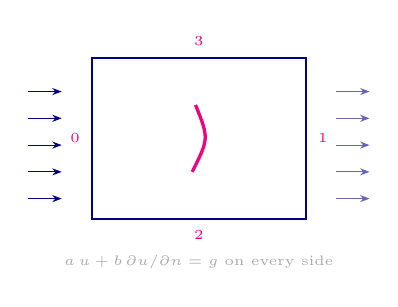
\begin{tikzpicture}[scale=0.85]
  \draw[NavyBlue,thick] (0,0) rectangle (3.2,2.4);
  \node[font=\tiny,text=RubineRed] at (-0.25,1.2) {0};
  \node[font=\tiny,text=RubineRed] at (3.45,1.2) {1};
  \node[font=\tiny,text=RubineRed] at (1.6,-0.25) {2};
  \node[font=\tiny,text=RubineRed] at (1.6,2.65) {3};
  \foreach \y in {0.3,0.7,...,2.1}{\draw[-{Stealth[length=1.2mm]},NavyBlue] (-0.95,\y) -- (-0.45,\y);}
  \foreach \y in {0.3,0.7,...,2.1}{\draw[-{Stealth[length=1.2mm]},NavyBlue!60] (3.65,\y) -- (4.15,\y);}
  \draw[RubineRed,very thick] (1.5,0.7) .. controls (1.75,1.2) .. (1.55,1.7);
  \node[font=\tiny,text=DarkGray] at (1.6,-0.65) {$a\,u + b\,\partial u/\partial n = g$ on every side};
\end{tikzpicture}}
\end{frame}

% 2
\begin{frame}{Learning goals}
\label{fr:goals}
\small By the end of this chapter you should be able to:
\begin{enumerate}
  \item write down a Robin boundary condition, say what the coefficients $a$, $b$ and $g$ mean, and say which pairs $(a,b)$ IBAMR's fluid solver actually accepts (only two);
  \item read and write the \code{VelocityBcCoefs\_0}, \code{\_1}, \code{\_2} blocks of an input file: the side numbering, the three keys per side, and the expressions in the quotes (variables, constants, functions, conditions);
  \item set up inflow, outflow, walls, moving walls, open sides and periodic sides, time-dependent and space-dependent conditions, and initial conditions, and know what IBAMR does and does not let you say about the pressure;
  \item size a rectangular domain and its grid: \code{domain\_boxes}, \code{x\_lo}, \code{x\_up}, levels, refinement ratio, coarsest and finest cell counts, patch sizes, and the divisibility rules that go with them;
  \item recognize the errors and warnings IBAMR prints for a broken boundary block, and the mistakes it accepts silently.
\end{enumerate}
\end{frame}

% 3
\begin{frame}{How this chapter was checked}
\label{fr:checked}
\begin{itemize}
  \item Every statement about what IBAMR does was checked against the 0.19.0 source: \code{INSStaggeredVelocityBcCoef.cpp} and \code{INSStaggeredPressureBcCoef.cpp} (what the coefficients do to the velocity and the pressure), \code{muParserRobinBcCoefs.cpp} (how the quoted expressions are read and which names they may use), \code{StaggeredStokesOpenBoundaryStabilizer.cpp}, \code{INSHierarchyIntegrator.cpp} and \code{AppInitializer.cpp} (the keys and warnings quoted).
  \item The error and warning messages are from short runs of IB/03 with deliberately broken boundary blocks (slides \ref{fr:err1}--\ref{fr:err2}), IBAMR 0.19.0 on one process; the script that made them is in the references.
  \item The figures are from runs of IB/03 and IB/02 in this series with their shipped inputs, rendered in VisIt 3.5.
  \item Where the 2013--2020 lectures said something else, the slide says so, and slides \ref{fr:changed}--\ref{fr:changed2} list the changes.
\end{itemize}
\begin{punchbox}
\small Slide numbers on the slides refer to this deck. The chapter numbers (5, 6, 8a, 11, 15, 16) refer to the other chapters of Part III.
\end{punchbox}
\end{frame}

% 4
\begin{frame}{Where to look things up}
\label{fr:lookup}
\small
\begin{itemize}
  \item \al{The examples}: every example in this series has its boundary and geometry blocks commented in \code{input2d} or \code{input3d}, and its README says what the conditions do. Start from the one closest to what you want (slides \ref{fr:leaf}--\ref{fr:scalar}).
  \item \al{The source}: \code{src/navier\_stokes/INSStaggeredVelocityBcCoef.cpp} (what $a$, $b$, $g$ do to the velocity), \code{INSStaggeredPressureBcCoef.cpp} (what they do to the pressure), \code{ibtk/src/boundary/physical\_boundary/muParserRobinBcCoefs.cpp} (how the quoted expressions are read), all unpacked by autoibamr under \code{tmp/unpack/IBAMR-<version>/}.
  \item \al{muParser}, the expression parser, has its own manual: \url{https://beltoforion.de/en/muparser/} (IBAMR bundles version 2 in \code{ibtk/contrib/muparser}).
  \item The grid blocks (\code{CartesianGeometry}, \code{GriddingAlgorithm}) belong to SAMRAI, which IBAMR bundles as IBSAMRAI2; the comments in the examples' input files are the practical reference.
  \item The IBAMR FAQ on the wiki, \url{https://github.com/IBAMR/IBAMR/wiki/FAQ}, and the users' group, \url{https://groups.google.com/g/ibamr-users}, where the pressure questions on slides \ref{fr:pressureq}--\ref{fr:ex0} were answered.
\end{itemize}
\end{frame}

% 5
\begin{frame}{The blocks of the input file this chapter covers}
\label{fr:blocksmap}
\scriptsize
\setlength{\tabcolsep}{4pt}
\begin{tabular}{@{}L{0.26\textwidth}L{0.40\textwidth}L{0.2\textwidth}@{}}
\toprule
Block & What it sets & Slides\\
\midrule
\code{VelocityBcCoefs\_0}, \code{\_1}, (\code{\_2}) & the boundary condition of one velocity component on every side of the box & \ref{fr:blocks}--\ref{fr:stab}\\
\code{VelocityInitialConditions}, \code{PressureInitialConditions} & the velocity (and, for output only, the pressure) at $t = 0$ & \ref{fr:ic}--\ref{fr:ic2}\\
\code{CartesianGeometry} & the index box of the coarsest grid, the physical corners of the domain, and which directions are periodic & \ref{fr:periodic}, \ref{fr:geom}\\
\code{GriddingAlgorithm} & the number of levels, the refinement ratio, the largest and smallest patch, the efficiency settings & \ref{fr:levels}--\ref{fr:gridding}\\
\code{StandardTagAndInitialize} and the tagging keys of the integrator block & which cells are refined: gradient detector or vorticity thresholds, the tag buffer, how often to regrid & \ref{fr:gridding}--\ref{fr:vort}\\
\code{IBHierarchyIntegrator} time keys & \code{dt\_max}, \code{end\_time}, \code{max\_integrator\_steps}, \code{grow\_dt} & \ref{fr:dt}--\ref{fr:outputs2}\\
the output keys (\code{viz\_dump\_interval}, \code{data\_dump\_interval}) & how often frames and data files are written, in time steps & \ref{fr:outputs}\\
\bottomrule
\end{tabular}

\vspace{2mm}
\small The physical constants at the top of the file (\code{MU}, \code{RHO}, the stiffnesses) are chapter 8a; the structure blocks (\code{IBStandardInitializer}) are chapter 6; the solver keys (\code{DELTA\_FUNCTION}, \code{CFL\_MAX}, \code{DT}) are chapter 5.
\end{frame}

% 6
\begin{frame}{Part I: boundary conditions}
\label{fr:part1}
\Large\color{NavyBlue} Part I: boundary conditions\par
\vspace{3mm}
\normalsize\color{black}
Robin conditions and what IBAMR makes of them; the side numbering; the \code{VelocityBcCoefs} blocks; the expressions in the quotes; walls, inflow, outflow, open and periodic sides; time- and space-dependent conditions; the examples; the pressure; initial conditions.
\vspace{3mm}

\small Part II (from slide \ref{fr:part2}) sizes the box and the grid.
\end{frame}

% 7
\begin{frame}{Robin boundary conditions}
\label{fr:robin}
\small Robin boundary conditions are a weighted combination of Dirichlet (value) and Neumann (derivative) conditions. If $\Omega$ is the domain on which the equation is solved and $\partial\Omega$ its boundary, the Robin condition is
\[
  a\,u + b\,\frac{\partial u}{\partial n} = g \quad\text{on } \partial\Omega,
\]
for constants $a$ and $b$, not both zero, and a given function $g$ on $\partial\Omega$. Here $\partial u/\partial n = \nabla u\cdot\mathbf{n}$ is the derivative along the \al{outward} unit normal $\mathbf{n}$.
\begin{itemize}
  \item $a = 1$, $b = 0$: a \al{Dirichlet} condition, $u = g$: the value is prescribed.
  \item $a = 0$, $b = 1$: a \al{Neumann} condition, $\partial u/\partial n = g$: the outward derivative is prescribed.
  \item both nonzero: a true Robin (mixed) condition, used for scalars (slide \ref{fr:scalar}) but not for the velocity (slide \ref{fr:accept}).
\end{itemize}
\vspace{1mm}
\begin{punchbox}
\small IBAMR asks for $a$, $b$ and $g$ separately for every side of the box and every velocity component, each as an expression in quotes. That is all a \code{VelocityBcCoefs} block is: $2\,\mathrm{NDIM}$ sides $\times$ three expressions.
\end{punchbox}
\end{frame}

% 8
\begin{frame}{Example: Robin conditions in one dimension}
\label{fr:oned}
\begin{columns}[T,onlytextwidth]
\begin{column}{0.56\textwidth}
\small In one dimension, with $\Omega = [0,1]$, the Robin condition becomes two conditions, one per end:
\[
  a\,u(0) - b\,u'(0) = g_0, \qquad a\,u(1) + b\,u'(1) = g_1 .
\]
Notice the change of sign in front of the derivative term. The outward normal at $x = 0$ points in the negative direction, so $\partial u/\partial n = -u'(0)$ there, while at $x = 1$ it points in the positive direction and $\partial u/\partial n = +u'(1)$.
\vspace{1mm}

\small The same happens on every side of a box: on a lower side (left, bottom, back) the outward normal is $-\mathbf{e}_d$, on an upper side it is $+\mathbf{e}_d$. IBAMR keeps track of this for you; you give $a$, $b$, $g$ and never type a minus sign for the normal.
\end{column}
\begin{column}{0.42\textwidth}
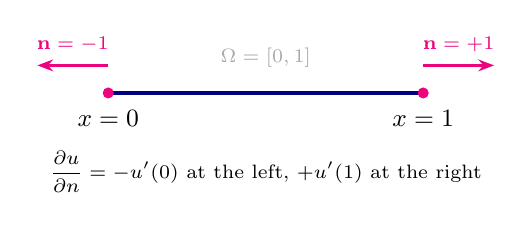
\begin{tikzpicture}[scale=1.0]
  \draw[NavyBlue,very thick] (0,0) -- (4,0);
  \fill[RubineRed] (0,0) circle (2pt); \fill[RubineRed] (4,0) circle (2pt);
  \node[below,font=\small] at (0,-0.1) {$x=0$}; \node[below,font=\small] at (4,-0.1) {$x=1$};
  \draw[-{Stealth[length=2mm]},RubineRed,thick] (0,0.35) -- (-0.9,0.35); \node[above,font=\scriptsize,text=RubineRed] at (-0.45,0.4) {$\mathbf{n}=-1$};
  \draw[-{Stealth[length=2mm]},RubineRed,thick] (4,0.35) -- (4.9,0.35); \node[above,font=\scriptsize,text=RubineRed] at (4.45,0.4) {$\mathbf{n}=+1$};
  \node[font=\scriptsize,text=DarkGray] at (2,0.45) {$\Omega=[0,1]$};
  \node[font=\scriptsize] at (2,-1.0) {$\dfrac{\partial u}{\partial n}=-u'(0)$ at the left, $+u'(1)$ at the right};
\end{tikzpicture}
\end{column}
\end{columns}
\end{frame}

% 9
\begin{frame}{No slip and Neumann in this notation, and a correction}
\label{fr:correction}
\small
\begin{itemize}
  \item \al{No-slip walls} (Dirichlet): $a = 1$, $b = 0$, $g = 0$ gives $u(0) = 0$ and $u(1) = 0$.
  \item \al{Neumann}: $a = 0$, $b = 1$, $g = 0$ gives $\partial u/\partial n = 0$ at both ends, that is $-u'(0) = 0$ and $u'(1) = 0$.
\end{itemize}
\vspace{1mm}
\begin{punchbox}
\small \al{A correction to the 2013--2020 slides.} They wrote the Neumann case as ``$a = 0$, $b = -1, 1$, $g = 0$'', with $b = -1$ at $x = 0$ and $b = +1$ at $x = 1$. That is the same condition written with $u'$ instead of $\partial u/\partial n$, and it is correct as mathematics. It is wrong as an input file: IBAMR's condition is written with the outward normal derivative, so $b = 1$ on \emph{both} ends, and the solver accepts only $b = 1$ (or $b = 0$). Typing $-1$ is an error (slide \ref{fr:accept}, tested on slide \ref{fr:err1}).
\end{punchbox}
\vspace{1mm}
\small Dirichlet and Neumann are the only two cases the fluid solver takes, and they mean rather more than ``value'' and ``derivative'' for a velocity component: slide \ref{fr:four}.
\end{frame}

% 10
\begin{frame}[fragile]{What IBAMR does with $a$, $b$ and $g$: only two choices}
\label{fr:accept}
\small For the velocity the coefficients are not used as a general Robin condition. The class that interprets them (\code{INSStaggeredVelocityBcCoef}) tests only whether $a = 1$ or $b = 1$:
\begin{lstlisting}[style=cpp]
const bool velocity_bc = IBTK::rel_equal_eps(alpha, 1.0);   // a == 1 : a velocity condition
const bool traction_bc = IBTK::rel_equal_eps(beta, 1.0);    // b == 1 : a traction condition
TBOX_ASSERT((velocity_bc || traction_bc) && !(velocity_bc && traction_bc));   // debug builds only
\end{lstlisting}
\begin{itemize}
  \item $(a, b) = (1, 0)$: \al{velocity condition}, $u_d = g$ on that side (an inflow profile, a wall, a moving wall).
  \item $(a, b) = (0, 1)$: \al{traction condition}, a condition on the stress rather than the velocity (an open side, a free-slip wall); what exactly depends on whether $d$ is the normal or a tangential component (slides \ref{fr:four}, \ref{fr:traction}).
  \item Anything else (both 1, both 0, $0.5$ and $0.5$, $-1$): a release build stops with \code{this statement should not be reached!} from \code{INSProjectionBcCoef.cpp}, a debug build with the assertion above. Tested on slide \ref{fr:err1}.
\end{itemize}
\begin{punchbox}
\small So $g$ is a velocity when $a = 1$ and a \emph{stress} (force per area, units of pressure) when $b = 1$. The same letter, two different physical quantities.
\end{punchbox}
\end{frame}

% 11
\begin{frame}{The four conditions a velocity component can carry}
\label{fr:four}
\scriptsize
\begin{tabular}{@{}L{0.12\textwidth}L{0.1\textwidth}L{0.36\textwidth}L{0.32\textwidth}@{}}
\toprule
$(a,b)$ & component & condition imposed & use it for\\
\midrule
$(1,0)$ & normal & $u_n = g$: the flow through the side is prescribed & inflow and outflow profiles; a wall ($g = 0$); a pulsing inlet\\
$(1,0)$ & tangential & $u_t = g$: the velocity along the side is prescribed & no slip ($g = 0$); a sliding lid or belt ($g = V$)\\
$(0,1)$ & normal & \code{TRACTION}: $-p + 2\mu\,\partial u_n/\partial n = g$; \code{PSEUDO\_TRACTION}: $-p = g$ & an open side where the flow chooses its own velocity; sets the pressure level there\\
$(0,1)$ & tangential & \code{TRACTION}: $\mu(\partial u_t/\partial n + \partial u_n/\partial t) = g$; \code{PSEUDO\_TRACTION}: $\mu\,\partial u_t/\partial n = g$ & a free-slip (shear-free) wall or open side with $g = 0$; a prescribed shear stress\\
\bottomrule
\end{tabular}

\vspace{2mm}
\small ``Normal'' means the component along the axis the side faces: $u_0$ ($x$) on sides 0 and 1, $u_1$ ($y$) on sides 2 and 3, $u_2$ ($z$) on sides 4 and 5 (numbering on slide \ref{fr:numbering}). The other components are tangential there. For the normal component with $(0,1)$ the velocity itself gets $\partial u_n/\partial n = 0$ (the source sets $\alpha = 0$, $\beta = 1$, $\gamma = 0$ for it) and $g$ goes into the pressure condition instead (slide \ref{fr:pressure}).
\vspace{1mm}

\small The choice between \code{TRACTION} (the default) and \code{PSEUDO\_TRACTION} is the key \code{traction\_bc\_type} in the \code{INSStaggeredHierarchyIntegrator} block (slide \ref{fr:traction}).
\end{frame}

% 12
\begin{frame}{Velocity conditions: walls, inflow, moving walls}
\label{fr:velocity}
\small With $(a, b) = (1, 0)$ on a side, $g$ is the velocity component there.
\begin{itemize}
  \item A \al{fixed wall}: $g = 0$ for all components on that side. The normal component $0$ means nothing flows through; the tangential components $0$ mean no slip.
  \item An \al{inflow}: the normal component $g = U$ (or a profile in the tangential coordinate, slide \ref{fr:space}, or a ramp in time, slide \ref{fr:time}); the tangential components $0$.
  \item A \al{moving wall} (lid, belt, sliding floor): the normal component $0$, a tangential component $g = V$. IB/08's lid (slide \ref{fr:ib08}) and the top and bottom of IB/03's box (slide \ref{fr:readblock}) are moving walls.
  \item An \al{outflow with a prescribed velocity}: the same as an inflow with the sign reversed. IB/03 and IBFE/10 prescribe the velocity on every side, including the outlet: a wind tunnel whose walls move with the stream.
\end{itemize}
\vspace{1mm}
\begin{punchbox}
\small If the normal velocity is prescribed on \emph{every} side (no open side, nothing periodic), the prescribed flux must balance: $\oint_{\partial\Omega} u_n\,dS = 0$, or the incompressibility constraint cannot be met. A uniform $U$ on all sides balances; a parabola in and the same parabola out balances; an inlet with closed walls everywhere else does not. Slide \ref{fr:compat} has the pressure side of this.
\end{punchbox}
\end{frame}

% 13
\begin{frame}[fragile]{Traction conditions: open sides}
\label{fr:traction}
\small With $(a, b) = (0, 1)$ on a side the velocity is not prescribed; the \al{stress} is. The two forms:
\begin{itemize}
  \item \code{TRACTION} (the default): the physical traction $\boldsymbol{\sigma}\mathbf{n}$ with $\boldsymbol{\sigma} = -p\mathbf{I} + \mu(\nabla\mathbf{u} + \nabla\mathbf{u}^T)$. Normal component: $-p + 2\mu\,\partial u_n/\partial n = g$. Tangential: $\mu(\partial u_t/\partial n + \partial u_n/\partial t) = g$.
  \item \code{PSEUDO\_TRACTION}: drops the transposed gradient. Normal: $-p = g$. Tangential: $\mu\,\partial u_t/\partial n = g$.
\end{itemize}
Choose with a key in the fluid integrator's block (any of the integrators; the default is \code{TRACTION}):
\begin{lstlisting}[style=input]
INSStaggeredHierarchyIntegrator {
   ...
   traction_bc_type = "PSEUDO_TRACTION"   // or "TRACTION" (default)
}
\end{lstlisting}
\begin{itemize}
  \item $g = 0$ on all components of a side is the usual \al{open (outflow) boundary}: zero normal stress, zero shear. The flow leaves (or enters) at whatever velocity the interior dictates, and the pressure there is $2\mu\,\partial u_n/\partial n \approx 0$.
  \item $g = 0$ on the tangential components only, with $u_n = 0$ prescribed, is a \al{free-slip wall}.
\end{itemize}
\end{frame}

% 14
\begin{frame}[fragile]{How the pressure gets its boundary condition}
\label{fr:pressure}
\small The pressure is not a state variable and has no block of its own. Its boundary condition is derived from the \emph{normal} velocity component's condition on each side (\code{INSStaggeredPressureBcCoef.cpp}):
\begin{lstlisting}[style=cpp]
// Normal velocity boundary conditions are converted into Neumann conditions for the pressure, and
// normal traction boundary conditions are converted into Dirichlet conditions for the pressure.
case TRACTION:        // -p + 2*mu*du_n/dx_n = g.
    // p^{n+1/2} = mu*du_n/dx_n^{n} + mu*du_n/dx_n^{n+1} - g^{n+1/2}.
case PSEUDO_TRACTION: // -p = g.
\end{lstlisting}
\begin{itemize}
  \item A \al{velocity} condition on the normal component gives a homogeneous Neumann condition for the pressure: the projection does not change the normal velocity at the boundary.
  \item A \al{traction} condition on the normal component gives a Dirichlet condition: the pressure at the boundary is $-g$ (pseudo-traction) or $2\mu\,\partial u_n/\partial n - g$ (traction, evaluated half at the old and half at the new time).
\end{itemize}
\begin{punchbox}
\small So an \al{outlet pressure} $p_{\mathrm{out}}$ is imposed by $a = 0$, $b = 1$, $g = -p_{\mathrm{out}}$ on the normal component of that side (and $g = 0$ on the tangential ones). Note the sign: $g$ is the normal traction, $-p$.
\end{punchbox}
\end{frame}

% 15
\begin{frame}{``Can I specify the pressure?'': then and now}
\label{fr:pressureq}
\small The 2013 lecture collected ``random notes'' on this question, because at the time the answer in the examples was no:
\begin{itemize}
  \item From Boyce Griffith, quoted on the 2013 slide: ``You cannot specify the pressure --- pressure is computed by the fluid solver --- but you can specify (in the code) a relationship between pressure and source/sink strength. You have to do all of this in the code --- i.e.\ there are not input parameters to set source strengths.''
  \item So pressure-driven flow was done with \al{sources and sinks} inside the domain (a model of the reservoirs), coupled to the computed pressure (slide \ref{fr:boyce}), or by prescribing the velocity.
\end{itemize}
\vspace{1mm}
\begin{punchbox}
\small \al{Now}: the traction condition of slides \ref{fr:traction}--\ref{fr:pressure} lets you set the pressure \emph{on a side of the box} directly from the input file, with $(a, b) = (0, 1)$ and $g = -p$ on the normal component. A pressure drop between an inlet and an outlet is two such sides with different $g$; the flow rate is then an output. Sources and sinks are still there (the \code{.source} file and \code{IBStandardSourceGen}, chapter 6) for reservoirs that are inside the box.
\end{punchbox}
\vspace{1mm}
\small Two cautions: an open inlet with traction conditions can admit flow in either direction, and an open outlet with backflow can go unstable; slide \ref{fr:stab} has the stabilizer for that. And with an open side the pressure level is fixed by the boundary, so \code{normalize\_pressure} must be \code{FALSE} (slide \ref{fr:compat}).
\end{frame}

% 16
\begin{frame}{Boyce's hints on relating pressure and source strength (2013)}
\label{fr:boyce}
\small Kept from the 2013 slide, because the reasoning still applies to any reservoir model you build in code. The question was how to pick the strength of a source for an inlet at pressure 2000 and two outlets at pressure 0.
\begin{itemize}
  \item The idea is a relationship $Q_{\mathrm{src}} = f(Q_{\mathrm{src}},\,P_{\mathrm{rsvr}} - P_{\mathrm{src}})$, where $Q_{\mathrm{src}}$ is the source/sink strength, $P_{\mathrm{src}}$ the pressure measured at the source (computed by the fluid solver) and $P_{\mathrm{rsvr}}$ the reservoir pressure specified as the external condition.
  \item A simple \al{resistive} connection: $Q_{\mathrm{src}} = (P_{\mathrm{rsvr}} - P_{\mathrm{src}})/R$. With $Q_{\mathrm{src}}$ counted as flow \emph{into} the domain (how IBAMR sets it up), the signs give inflow when $P_{\mathrm{src}} < P_{\mathrm{rsvr}}$.
  \item In practice a bit of delay is needed for stability, by adding \al{inertance}: $R\,Q_{\mathrm{src}} + L\,\dot{Q}_{\mathrm{src}} = P_{\mathrm{rsvr}} - P_{\mathrm{src}}$. His guess for why: the interior is coupled to the reservoirs explicitly in time; an implicit coupling could use a purely resistive connection.
\end{itemize}
\vspace{1mm}
\small Flow meters and pressure gauges were built out of ``rings'' of immersed-boundary points: the flow is the total velocity flux through a web spanning the ring, and the pressure is read at the ring's centroid. That is still how the \code{.inst} file works (chapter 6, \code{IBInstrumentPanel}).
\end{frame}

% 17
\begin{frame}[fragile]{The same note: initial conditions, and where the example is}
\label{fr:ex0}
\small Also quoted on the 2013 slide, from the users' group, about a non-uniform incoming velocity profile (``linear increasing in z-direction'') as the initial state:
\begin{quote}\footnotesize
``I think you are asking about setting up initial conditions. It is pretty straightforward to do this; see IBAMR/examples/navier\_stokes/ex0 for an example. There are several different input files that set up nontrivial initial conditions for the velocity and pressure. (Note that the initial condition for the pressure is only used for output purposes, since the pressure is not a state variable.)'' --- Boyce
\end{quote}
\code{navier\_stokes/ex0} is still in the 0.19.0 tree. Its input file defines the exact solution as strings at the top (\code{U = "1 - 2*(cos(2*PI*(X\_0-t))*...)"}, likewise \code{V} and \code{P}) and refers to them by name, without quotes, inside the blocks:
\begin{lstlisting}[style=inputtiny]
VelocityInitialConditions {
   nu = MU/RHO
   function_0 = U          // the input parser substitutes the string U; muParser then reads it
   function_1 = V
}
PressureInitialConditions {
   nu = MU/RHO
   function = P            // one function, not function_0: the pressure is a scalar
}
\end{lstlisting}
Slides \ref{fr:ic}--\ref{fr:ic2} have the initial-condition blocks of the examples in this series.
\end{frame}

% 18
\begin{frame}{IBAMR boundary numbering}
\label{fr:numbering}
\begin{columns}[T,onlytextwidth]
\begin{column}{0.5\textwidth}
\small Look in any \code{input2d} or \code{input3d}: each side of the box has a number, used as the suffix of the keys.
\begin{itemize}
  \item 2D: \al{0} = $x$ lower (left), \al{1} = $x$ upper (right), \al{2} = $y$ lower (bottom), \al{3} = $y$ upper (top).
  \item 3D: add \al{4} = $z$ lower and \al{5} = $z$ upper.
\end{itemize}
The rule behind it: side $= 2\,\times$ axis $+$ (0 for the lower end, 1 for the upper end), so axis $=$ side$/2$ and lower/upper $=$ side mod 2. The source uses exactly this (\code{axis = location\_index / 2; side = location\_index \% 2}).
\vspace{1mm}

\small ``Lower'' and ``upper'' refer to the coordinate value, not to the picture: in 3D the ``bottom'' of a box that stands along $z$ is side 4, and in 2D the ``floor'' is side 2.
\end{column}
\begin{column}{0.48\textwidth}
\centering
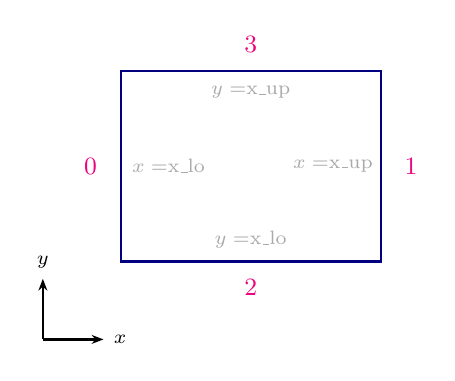
\begin{tikzpicture}[scale=1.1]
  \draw[NavyBlue,thick] (0,0) rectangle (3,2.2);
  \node[font=\small,text=RubineRed] at (-0.35,1.1) {0};
  \node[font=\small,text=RubineRed] at (3.35,1.1) {1};
  \node[font=\small,text=RubineRed] at (1.5,-0.3) {2};
  \node[font=\small,text=RubineRed] at (1.5,2.5) {3};
  \node[font=\scriptsize,text=DarkGray] at (0.55,1.1) {$x=$\code{x\_lo}};
  \node[font=\scriptsize,text=DarkGray] at (2.45,1.1) {$x=$\code{x\_up}};
  \node[font=\scriptsize,text=DarkGray] at (1.5,0.25) {$y=$\code{x\_lo}};
  \node[font=\scriptsize,text=DarkGray] at (1.5,1.95) {$y=$\code{x\_up}};
  \draw[-{Stealth[length=1.5mm]},thick] (-0.9,-0.9) -- (-0.2,-0.9) node[right,font=\scriptsize] {$x$};
  \draw[-{Stealth[length=1.5mm]},thick] (-0.9,-0.9) -- (-0.9,-0.2) node[above,font=\scriptsize] {$y$};
\end{tikzpicture}
\vspace{1mm}

\scriptsize
\setlength{\tabcolsep}{3pt}
\begin{tabular}{@{}lccc@{}}
\toprule
axis & lower side & upper side & normal component\\
\midrule
$x$ (0) & 0 & 1 & $u_0$: \code{VelocityBcCoefs\_0}\\
$y$ (1) & 2 & 3 & $u_1$: \code{VelocityBcCoefs\_1}\\
$z$ (2) & 4 & 5 & $u_2$: \code{VelocityBcCoefs\_2}\\
\bottomrule
\end{tabular}
\end{column}
\end{columns}
\end{frame}

% 19
\begin{frame}[fragile]{The \code{VelocityBcCoefs} blocks: one per component, three keys per side}
\label{fr:blocks}
\begin{columns}[T,onlytextwidth]
\begin{column}{0.46\textwidth}
\footnotesize There is one block per velocity component: \code{VelocityBcCoefs\_0} for $u$ ($x$), \code{\_1} for $v$ ($y$), and in 3D \code{\_2} for $w$ ($z$). Each block holds, for every side $s$, the three strings \code{acoef\_function\_s}, \code{bcoef\_function\_s}, \code{gcoef\_function\_s}.
\vspace{1mm}

\footnotesize The block on the right (from the 2013--2020 slides) sets the $y$-velocity to zero on all four sides: no flow through the top and bottom, no slip along the left and right. The $x$-component block decides whether anything flows at all.
\vspace{1mm}

\footnotesize \code{main.cpp} reads the blocks by name, so the names are fixed: \code{"VelocityBcCoefs\_" << d} for $d = 0,\ldots,\mathrm{NDIM}-1$, each passed to a \code{muParserRobinBcCoefs} object (IB/03's \code{main.cpp}, lines 229--236). What happens when a block is missing: next slide.
\end{column}
\begin{column}{0.52\textwidth}
\begin{lstlisting}[style=inputtiny]
VelocityBcCoefs_1 {   // y-component of the velocity
   acoef_function_0 = "1.0"
   acoef_function_1 = "1.0"
   acoef_function_2 = "1.0"
   acoef_function_3 = "1.0"

   bcoef_function_0 = "0.0"
   bcoef_function_1 = "0.0"
   bcoef_function_2 = "0.0"
   bcoef_function_3 = "0.0"

   gcoef_function_0 = "0.0"
   gcoef_function_1 = "0.0"
   gcoef_function_2 = "0.0"
   gcoef_function_3 = "0.0"
}
\end{lstlisting}
\end{column}
\end{columns}
\end{frame}

% 19b
\begin{frame}[fragile]{How the blocks reach the solver, and what a missing block does}
\label{fr:blocks2}
\begin{columns}[T,onlytextwidth]
\begin{column}{0.52\textwidth}
\begin{lstlisting}[style=cpptiny]
// IB/03 main.cpp, lines 211-236 (condensed)
const IntVector<NDIM>& periodic_shift = grid_geometry->getPeriodicShift();
vector<RobinBcCoefStrategy<NDIM>*> u_bc_coefs(NDIM);
if (periodic_shift.min() > 0)          // fully periodic: no blocks needed
{
    for (unsigned int d = 0; d < NDIM; ++d) u_bc_coefs[d] = nullptr;
}
else
{
    for (unsigned int d = 0; d < NDIM; ++d)
    {
        ostringstream bc_coefs_db_name_stream;
        bc_coefs_db_name_stream << "VelocityBcCoefs_" << d;
        u_bc_coefs[d] = new muParserRobinBcCoefs(
            bc_coefs_name, app_initializer->getComponentDatabase(bc_coefs_db_name), grid_geometry);
    }
    navier_stokes_integrator->registerPhysicalBoundaryConditions(u_bc_coefs);
}
\end{lstlisting}
\end{column}
\begin{column}{0.46\textwidth}
\scriptsize
\begin{itemize}
  \item In a \al{fully periodic} box (every entry of \code{periodic\_dimension} is 1) the blocks are not read at all; the integrator gets no boundary objects.
  \item Otherwise one \code{muParserRobinBcCoefs} is built per component from the block of that name and the set is registered with the fluid integrator; the IB and IBFE \code{main.cpp} files in this series all contain this loop.
  \item A \al{missing block} is not fatal by itself: \code{AppInitializer::getComponentDatabase} prints \code{WARNING: ... Database corresponding to component `VelocityBcCoefs\_1' not found in input} and hands over an empty database, so every side then gets the missing-key warning of slide \ref{fr:err2} and $a = b = 0$, which the fluid solver rejects at its first use (slide \ref{fr:accept}). Both warnings are in the log file.
\end{itemize}
\end{column}
\end{columns}
\end{frame}

% 20
\begin{frame}[fragile]{Reading a block: the $x$-velocity of the tethered leaf (IB/03)}
\label{fr:readblock}
\begin{columns}[T,onlytextwidth]
\begin{column}{0.5\textwidth}
\begin{lstlisting}[style=inputtiny]
VelocityBcCoefs_0 {       // x-component
   U_FLOW = V             // from the top of the file

   acoef_function_0 = "1.0"
   acoef_function_1 = "1.0"
   acoef_function_2 = "1.0"
   acoef_function_3 = "1.0"

   bcoef_function_0 = "0.0"
   bcoef_function_1 = "0.0"
   bcoef_function_2 = "0.0"
   bcoef_function_3 = "0.0"

   gcoef_function_0 = "U_FLOW*tanh(2*t)"
   gcoef_function_1 = "U_FLOW*tanh(2*t)"
   gcoef_function_2 = "U_FLOW*tanh(2*t)"
   gcoef_function_3 = "U_FLOW*tanh(2*t)"
}
\end{lstlisting}
\end{column}
\begin{column}{0.48\textwidth}
\small Line by line, the first half:
\begin{itemize}
  \item \code{U\_FLOW = V}: a constant for the expressions below, copied from \code{V = 0.1} at the top of the file (why the copy is needed: slide \ref{fr:blockconst}).
  \item all $a = 1$, $b = 0$: every side prescribes the $x$-velocity (a velocity condition, slide \ref{fr:accept}); nothing here is a wall or an open side by itself. What each side does is decided by $g$, on the next slide.
  \item the four lines of each key are the four sides of slide \ref{fr:numbering}, in the order left, right, bottom, top.
\end{itemize}
\end{column}
\end{columns}
\end{frame}

% 21
\begin{frame}[fragile]{Reading a block, continued: what $g$ makes of each side}
\label{fr:readblock2}
\begin{columns}[T,onlytextwidth]
\begin{column}{0.5\textwidth}
\begin{lstlisting}[style=input]
   gcoef_function_0 = "U_FLOW*tanh(2*t)"   // left:   inflow
   gcoef_function_1 = "U_FLOW*tanh(2*t)"   // right:  outflow
   gcoef_function_2 = "U_FLOW*tanh(2*t)"   // bottom: sliding wall
   gcoef_function_3 = "U_FLOW*tanh(2*t)"   // top:    sliding wall
\end{lstlisting}
\begin{lstlisting}[style=input]
VelocityBcCoefs_1 {       // y-component: all zero
   acoef_function_0 = "1.0"   ...
   bcoef_function_0 = "0.0"   ...
   gcoef_function_0 = "0.0"   ...
}
\end{lstlisting}
\end{column}
\begin{column}{0.48\textwidth}
\small
\begin{itemize}
  \item $g = $\code{U\_FLOW*tanh(2*t)} on all four sides: the $x$-velocity rises smoothly from $0$ to $U$ (96\% of it by $t = 1$ s, slide \ref{fr:time}). On side 0 that is inflow, on side 1 outflow, on sides 2 and 3 (where $u$ is tangential) a wall sliding at the stream speed.
  \item the $y$-block is all zeros: nothing crosses the top or bottom, and the ends have no $y$-velocity.
  \item The course version wrote \code{0.1*tanh(2*t)} on each line; the constant makes the speed a one-line change at the top of the file.
\end{itemize}
\small The result is the uniform stream of slide \ref{fr:leaf}.
\end{column}
\end{columns}
\end{frame}

% 22
\begin{frame}{What goes in the quotes: variables and built-in constants}
\label{fr:vars}
\small Each string is a muParser expression, evaluated at every boundary point at every time step. \code{muParserRobinBcCoefs.cpp} defines these names (0.19.0):
\vspace{1mm}

\scriptsize
\begin{tabular}{@{}L{0.3\textwidth}L{0.6\textwidth}@{}}
\toprule
Name(s) & Meaning\\
\midrule
\code{t}, \code{T} & the current time\\
\code{X\_0}, \code{X\_1}, \code{X\_2} (also \code{X0}, \code{x\_0}, \code{x0}) & the coordinates $x$, $y$, $z$ of the boundary point being evaluated. On side 0 or 1, \code{X\_0} is constant (it is \code{x\_lo} or \code{x\_up}) and \code{X\_1} varies along the side\\
\code{pi}, \code{Pi}, \code{PI} & $3.14159\ldots$ (so a \code{PI} key in the block, as IB/02 has, just redefines the same value)\\
\code{X\_LOWER\_0}, \code{X\_UPPER\_0}, \ldots\ (also \code{X\_lower0}, \code{XLower\_0}, \code{xlower0}, \ldots) & the physical corners of the domain from \code{CartesianGeometry}, in every spelling the author could think of\\
any numeric key in the block (\code{U\_FLOW = 0.1}, \code{f = 5}, \code{N = 32}) & a constant (slide \ref{fr:blockconst})\\
\bottomrule
\end{tabular}

\vspace{2mm}

\small The 2013--2020 lectures listed \code{t}, \code{X\_0}, \code{X\_1}, \code{X\_2}; the rest is from the source. The normal vector is not available as a variable; you know it from the side number.
\end{frame}

% 23
\begin{frame}{What goes in the quotes: functions and operators}
\label{fr:funcs}
\small muParser 2 (bundled in \code{ibtk/contrib/muparser}) provides:
\begin{itemize}
  \item \al{functions}: \code{sin cos tan asin acos atan atan2 sinh cosh tanh asinh acosh atanh exp ln log log2 log10 sqrt abs sign rint}, and the multi-argument \code{min max sum avg}.
  \item \al{arithmetic}: \code{+ - * / \^{}} (power), unary minus, parentheses.
  \item \al{comparison and logic}: \code{< <= > >= == !=}, \code{\&\&}, \code{||}, \code{!}; true is $1$ and false is $0$, so \code{(t < 1)*t} is a valid piecewise expression.
  \item \al{the conditional} \code{cond ? a : b} (slide \ref{fr:ternary}).
\end{itemize}
\vspace{1mm}
\begin{punchbox}
\small Numbers are read as decimals: \code{1} and \code{1.0} are the same. Division of two constants is floating-point division (\code{1/2} is $0.5$); the \code{int()} seen at the top of the input files (\code{VIZ\_INTERVAL = int(END\_TIME/(50*DT))}) is SAMRAI's input-file arithmetic, not muParser's, and does not exist inside the quotes.
\end{punchbox}
\vspace{1mm}
\small A name muParser does not know stops the run at start-up with \code{Unexpected token "<name>" found at position <n>} and the offending expression printed under it (tested on slide \ref{fr:err1}). The manual, \url{https://beltoforion.de/en/muparser/}, has the full list.
\end{frame}

% 24
\begin{frame}[fragile]{Constants defined in the block, and the trap at the top of the file}
\label{fr:blockconst}
\small Any key in the block whose value is a number becomes a constant the expressions can use (the constructor copies every double and integer key into the parser). That is how the examples parametrize their conditions:
\begin{lstlisting}[style=inputtiny]
VelocityBcCoefs_0 {
   U_FLOW = V                 // IB/03: the stream speed, from V at the top of the file
   PI = 3.141592653589793     // IB/02: also f = 5, d = 1.0, Y_high = 0.5*d, Y_low = -0.5*d
   U0 = U_FLOW                // IBFE/10: "copied here because the expressions can use only
   V_LID = V                  // IB/08:   constants defined in their block"
   SHEAR = SHEAR_START
   ...
\end{lstlisting}
\begin{punchbox}
\footnotesize \al{The trap}: a name defined at the top level of the input file (\code{V = 0.1}, \code{L = 1.0}) is \emph{not} visible inside the quotes. The input file's own arithmetic (\code{U\_FLOW = V}) can see it; muParser, which reads the quoted string later, cannot. Writing \code{"V*tanh(2*t)"} with \code{V} only at the top stops the run with \code{Unexpected token "V" found at position 0} (tested, slide \ref{fr:err1}). Copy the value into the block, as every example does.
\end{punchbox}
\footnotesize The same rule holds for \code{VelocityInitialConditions} and the scalar blocks, which use the same parser (\code{muParserCartGridFunction}). The exception is a top-level \emph{string}: \code{function\_0 = U} without quotes, as in \code{navier\_stokes/ex0} (slide \ref{fr:ex0}), pastes the string in before muParser sees it.
\end{frame}

% 25
\begin{frame}[fragile]{Conditions: the \code{if()} of the old lectures and the \code{? :} of today}
\label{fr:ternary}
\begin{columns}[T,onlytextwidth]
\begin{column}{0.5\textwidth}
\small The 2013--2020 slides taught in-line if-statements:
\begin{lstlisting}[style=data]
if( logical statement, a, b )
\end{lstlisting}
\small ``if the logical statement is true, do \code{a}; if false, do \code{b}'', nested as \code{if(s1, a, if(s2, b, c))}. That was muParser 1's syntax. The bundled muParser 2 has no \code{if} function; running the course's pulsatile input stops at start-up with
\begin{lstlisting}[style=tiny]
muParserRobinBcCoefs::setDataOnPatch():
  error: Unexpected token "if" found at position 0.
  in:    if(t<1, U_FLOW*t, U_FLOW)
\end{lstlisting}
\small (An \code{if} does appear in muParser's source, in its integer-only parser \code{muParserInt.cpp}; IBAMR does not use that parser.)
\end{column}
\begin{column}{0.48\textwidth}
\small Write the condition as a \al{ternary} instead:
\begin{lstlisting}[style=data]
(logical statement) ? a : b
\end{lstlisting}
\small Same meaning: if the statement is true the value is \code{a}, otherwise \code{b}. Nested:
\begin{lstlisting}[style=data]
(s1) ? a : ((s2) ? b : c)
\end{lstlisting}
\small ``if s1 then a, else if s2 then b, else c''. Put parentheses around the condition and around a nested ternary; muParser's precedence rules for \code{?:} are easy to get wrong otherwise.
A ramp that reaches $U$ at $t = 1$ and stays there:
\begin{lstlisting}[style=data]
(t < 1) ? U_FLOW*t : U_FLOW
\end{lstlisting}
\small The products-of-logicals form \code{(t<1)*U\_FLOW*t + (t>=1)*U\_FLOW} gives the same value and also works.
\end{column}
\end{columns}
\end{frame}

% 26
\begin{frame}[fragile]{The pulsatile-channel condition, before and after}
\label{fr:pulsexpr}
\small The course's \code{4-Example\_2DPulsatileChannelFlow} (now IB/02) prescribed, on the left and right ends, a parabolic profile across the channel ($|y| < d/2$), zero outside it, with a peak that pulses in time:
\begin{lstlisting}[style=inputtiny]
// course version (muParser 1 syntax; fails in 0.16 and 0.19 with: Unexpected token "if" found at position 0.)
gcoef_function_0 = "if( X_1 <= -0.5*d,0.0,if( X_1 >= 0.5*d,0.0,4.0/(d*d)*(0.5 + 0.5*sin(2*PI*f*t))*( (0.25*d*d) - X_1*X_1 ) ) )"
\end{lstlisting}
\begin{lstlisting}[style=inputtiny]
// IB/02 as shipped in this series (ternary syntax); the same string on side 1 (gcoef_function_1)
gcoef_function_0 = "(X_1 <= -0.5*d) ? 0.0 : ((X_1 >= 0.5*d) ? 0.0 : 4.0/(d*d)*(0.5 + 0.5*sin(2*PI*f*t))*((0.25*d*d) - X_1*X_1))"
\end{lstlisting}
\small Reading it from the outside in:
\begin{itemize}
  \item below the channel ($y \le -d/2$): $0$; above it ($y \ge d/2$): $0$;
  \item inside: $\dfrac{4}{d^2}\,\bigl(\tfrac12 + \tfrac12\sin 2\pi f t\bigr)\bigl(\tfrac{d^2}{4} - y^2\bigr)$, a parabola with peak $1$ at $y = 0$, scaled by a factor that swings between $0$ and $1$ at $f = 5$ Hz.
\end{itemize}
\small The constants \code{d}, \code{f} and \code{PI} are defined in the block (slide \ref{fr:blockconst}). Slide \ref{fr:ib02b} draws the profile; slide \ref{fr:ib02} shows the whole block.
\end{frame}

% 27
\begin{frame}{Time-dependent conditions: ramps and oscillations}
\label{fr:time}
\small Any expression may use \code{t}. The patterns in the examples:
\begin{itemize}
  \item \al{a smooth start}, \code{U*tanh(2*t)}: $0$ at $t = 0$, 76\% of $U$ at $t = 0.5$, 96\% at $t = 1$, 99.9\% at $t = 2$. IB/03, IB/08 and IBFE/10 all use it.
  \item \al{a pulse}, \code{0.5 + 0.5*sin(2*PI*f*t)}: between $0$ and $1$ with period $1/f$; IB/02. Replace by \code{sin(2*PI*f*t)} for a flow that reverses.
  \item \al{a linear ramp that stops}, \code{(t < 1) ? U*t : U}, or a switched-on constant, \code{(t > t\_on) ? U : 0} (slide \ref{fr:ternary}).
  \item IB/08's lid, \code{V\_LID*(SHEAR + (1 - SHEAR)*tanh(2*t))}: with the block constant \code{SHEAR = 0} this is the tanh ramp; with \code{SHEAR = 1} the lid moves at full speed from the first step (used together with a matching initial condition, slide \ref{fr:ic2}).
\end{itemize}
\vspace{1mm}
\begin{punchbox}
\small \al{Why ramp?} The fluid starts at rest (slide \ref{fr:ic}). A boundary velocity that jumps to $U$ at $t = 0$ is an impulsive start: the first steps see an enormous pressure and a velocity field that is not divergence-free near the boundary, the structure gets a hammer blow, and with \code{error\_on\_dt\_change} the run may stop at once. A $\tanh(2t)$ ramp costs about a second of simulated time and avoids all of that. Chapter 16 (what can go wrong) returns to this.
\end{punchbox}
\end{frame}

% 28
\begin{frame}{Space-dependent conditions: profiles along a side}
\label{fr:space}
\begin{columns}[T,onlytextwidth]
\begin{column}{0.55\textwidth}
\small On a side, the coordinate along the side is a variable: \code{X\_1} on sides 0 and 1 (the left and right ends), \code{X\_0} on sides 2 and 3; in 3D two coordinates vary on each face.
\begin{itemize}
  \item \al{Poiseuille} inflow across a channel of width $d$ centred on $y = 0$: $u = U_{\max}\,(1 - 4y^2/d^2)$, which is the IB/02 parabola, $\frac{4}{d^2}(\frac{d^2}{4} - y^2)$, times $U_{\max}$.
  \item A \al{plug} in a window: \code{(X\_1 > Y\_low \&\& X\_1 < Y\_high) ? U : 0}.
\end{itemize}
\small The profile is evaluated at the cell faces of every level that touches the boundary, so it is as sharp as the finest grid there. More profiles on the next slide.
\end{column}
\begin{column}{0.43\textwidth}
\centering
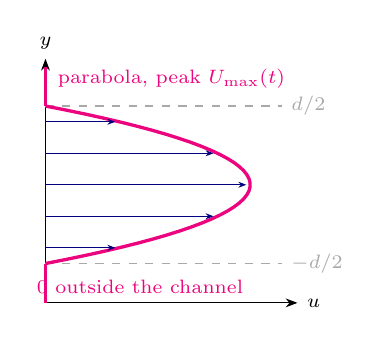
\begin{tikzpicture}[scale=1.0]
  \draw[-{Stealth[length=1.5mm]}] (0,-1.5) -- (0,1.6) node[above,font=\scriptsize] {$y$};
  \draw[-{Stealth[length=1.5mm]}] (0,-1.5) -- (3.2,-1.5) node[right,font=\scriptsize] {$u$};
  \draw[dashed,DarkGray] (0,1) -- (3,1) node[right,font=\scriptsize,text=DarkGray] {$d/2$};
  \draw[dashed,DarkGray] (0,-1) -- (3,-1) node[right,font=\scriptsize,text=DarkGray] {$-d/2$};
  \draw[RubineRed,very thick] plot[domain=-1:1,samples=40] ({2.6*(1-\x*\x)},\x);
  \draw[RubineRed,very thick] (0,1) -- (0,1.5); \draw[RubineRed,very thick] (0,-1) -- (0,-1.5);
  \foreach \y in {-0.8,-0.4,0,0.4,0.8}{\draw[-{Stealth[length=1mm]},NavyBlue] (0,\y) -- ({2.6*(1-\y*\y)-0.05},\y);}
  \node[font=\scriptsize,text=RubineRed] at (1.6,1.35) {parabola, peak $U_{\max}(t)$};
  \node[font=\scriptsize,text=RubineRed] at (1.2,-1.3) {$0$ outside the channel};
\end{tikzpicture}
\end{column}
\end{columns}
\end{frame}

% 29
\begin{frame}{Space-dependent conditions: more profiles}
\label{fr:space2}
\begin{columns}[T,onlytextwidth]
\begin{column}{0.55\textwidth}
\footnotesize
\begin{itemize}
  \item A \al{linear shear}: \code{U*(X\_1 - X\_LOWER\_1)/(X\_UPPER\_1 - X\_LOWER\_1)}, using the built-in corner constants of slide \ref{fr:vars}; $0$ at the bottom of the side, $U$ at the top.
  \item A \al{smoothed window} to avoid the sharp corner of the plug: multiply $U$ by \code{0.5*(1 + tanh((X\_1 - Y\_low)/w))*0.5*(1 - tanh((X\_1 - Y\_high)/w))} with $w$ a few cells wide.
  \item A \al{3D parabola} on side 0 of a square duct: \code{U*(1 - 4*X\_1*X\_1/(d*d))*(1 - 4*X\_2*X\_2/(d*d))}, which is zero on all four duct walls.
  \item A \al{travelling} profile: any function of \code{X\_1 - c*t}; a wave on the side.
\end{itemize}
\footnotesize Whatever the profile, the normal velocity on an inflow side should go to zero at the corners of the box where it meets a no-slip wall, or the corner cell has a discontinuous velocity. The parabola does; the plug does not, hence the window.
\end{column}
\begin{column}{0.43\textwidth}
\centering
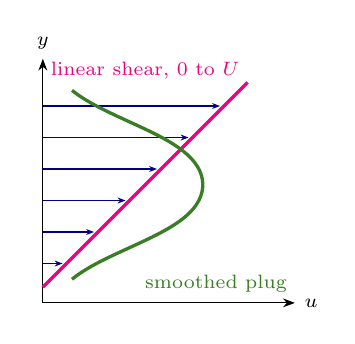
\begin{tikzpicture}[scale=1.0]
  \draw[-{Stealth[length=1.5mm]}] (0,-1.5) -- (0,1.6) node[above,font=\scriptsize] {$y$};
  \draw[-{Stealth[length=1.5mm]}] (0,-1.5) -- (3.2,-1.5) node[right,font=\scriptsize] {$u$};
  \draw[RubineRed,very thick] (0,-1.3) -- (2.6,1.3);
  \foreach \y in {-1.0,-0.6,-0.2,0.2,0.6,1.0}{\draw[-{Stealth[length=1mm]},NavyBlue] (0,\y) -- ({(\y+1.3)-0.05},\y);}
  \node[font=\scriptsize,text=RubineRed] at (1.3,1.45) {linear shear, $0$ to $U$};
  \draw[OliveGreen,very thick] plot[domain=-1.2:1.2,samples=60] ({2.2*0.25*(1+tanh((\x+0.8)*2))*(1-tanh((\x-0.8)*2))},\x);
  \node[font=\scriptsize,text=OliveGreen] at (2.2,-1.25) {smoothed plug};
\end{tikzpicture}
\end{column}
\end{columns}
\end{frame}

% 30
\begin{frame}{Example: a tethered leaf in a stream (IB/03)}
\label{fr:leaf}
\begin{columns}[T,onlytextwidth]
\begin{column}{0.5\textwidth}
\small The 2013--2020 ``tethered beam in flow'' (\code{4-Example\_2DTetheredBeam}): a beam tethered at its centre is placed in a flow that is ramped from $0$ to $0.1$ by setting \emph{all} boundary conditions to $U(t)$ in $x$ and $0$ in $y$, with $U$ a function of time so that the flow accelerates from rest.
\begin{itemize}
  \item side 0 (left): inflow at $U\tanh 2t$;
  \item side 1 (right): outflow at the same speed;
  \item sides 2 and 3: walls sliding at the stream speed (no boundary layer, so the box can be small);
  \item $v = 0$ everywhere on the boundary.
\end{itemize}
\small Box $1\times1$ m, $\mu = 4$, $\rho = 1000$, finest grid $512^2$.
\end{column}
\begin{column}{0.48\textwidth}
\centering
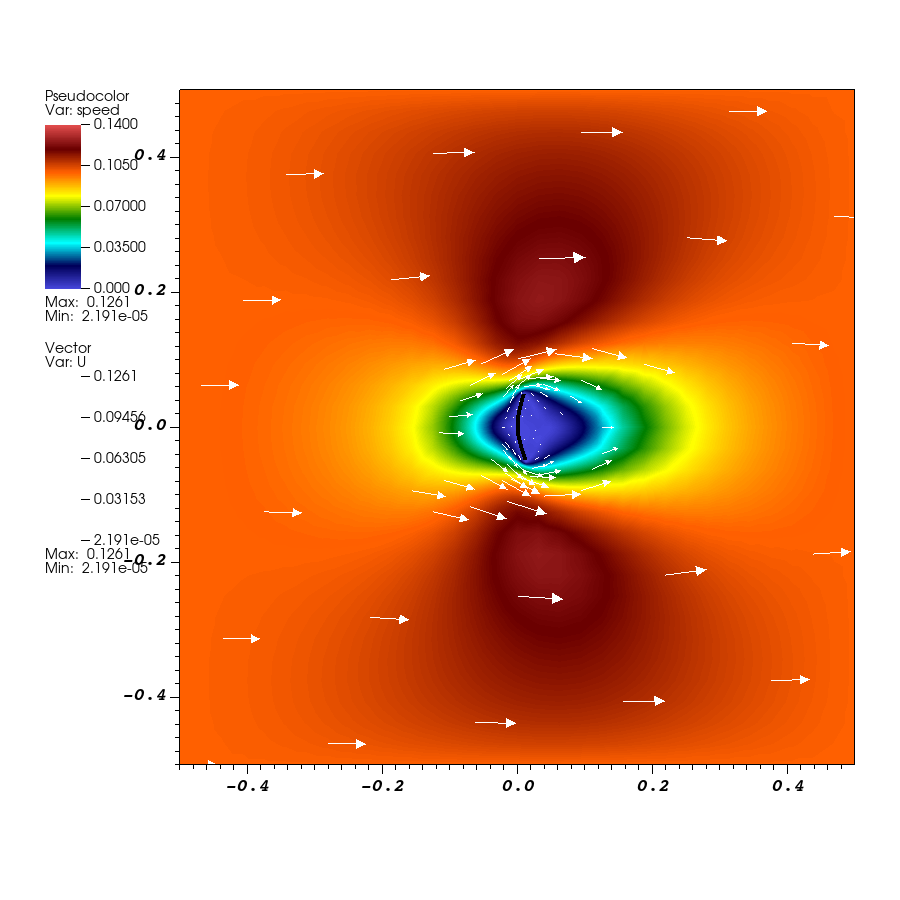
\includegraphics[height=0.66\textheight]{ch7-leaf-box-speed}
\end{column}
\end{columns}
\sourcecredit{IB/03 run with IBAMR 0.19.0 (default input, 2 s); VisIt 3.5, \code{wsl/final/visit\_ch7.sh}. Speed $|\mathbf{u}|$ from 0 (blue) to 0.14 m/s (dark red), vectors every 40th cell, the leaf in black.}
\end{frame}

% 31
\begin{frame}{The leaf in its box: reading the picture}
\label{fr:leaf2}
\begin{columns}[T,onlytextwidth]
\begin{column}{0.48\textwidth}
\centering
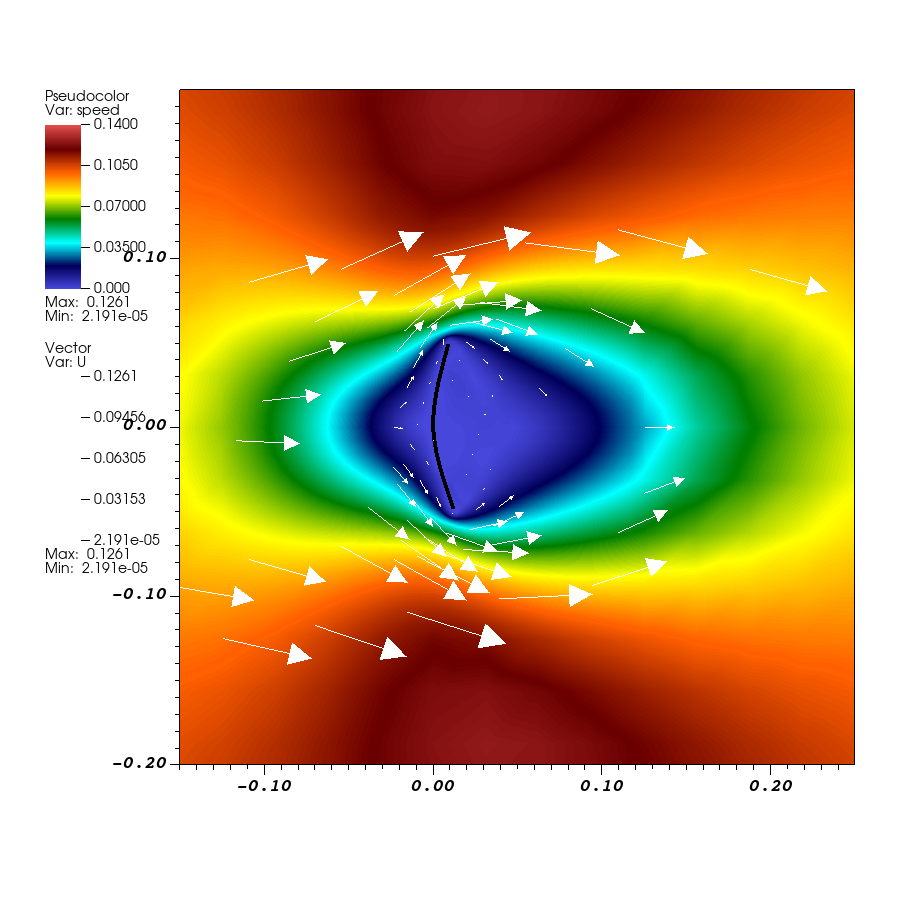
\includegraphics[height=0.66\textheight]{ch7-leaf-near-speed}
\end{column}
\begin{column}{0.5\textwidth}
\small The previous picture is speed at $t = 2$ s, with velocity vectors and the leaf in black. The stream is uniform away from the leaf; the fluid is slowed in front of and behind it and speeds up around it. Close up (left): the stagnant region (dark blue) in front and behind, the two fast lobes (red) above and below where the fluid squeezed past the leaf is faster than the stream, and the leaf bent slightly downstream by the flow.
\vspace{1mm}

\small At the box edges the vectors are all the same length and horizontal: that is the boundary condition, $u = U\tanh 4 \approx 0.1$, $v = 0$, on all four sides at this time.
\end{column}
\end{columns}
\sourcecredit{Same run and script as the previous slide, window $-0.15 \le x \le 0.25$, $-0.2 \le y \le 0.2$.}
\end{frame}

% 32
\begin{frame}{The leaf: what the prescribed walls mean, and first experiments}
\label{fr:leaf3}
\small Because the velocity is prescribed on all four sides, IB/03's box is a wind tunnel whose walls move with the free stream:
\begin{itemize}
  \item the inflow and outflow fluxes balance exactly (the same $U$ on sides 0 and 1), as slide \ref{fr:velocity} requires;
  \item the top and bottom do not grow boundary layers, so the leaf's wake is not confined by them as it would be by no-slip walls;
  \item but the outlet is \emph{forced} to be uniform: a wake that reaches side 1 is squeezed back to $U$ there. The box must be long enough, or the outlet must be open (slides \ref{fr:traction}, \ref{fr:open}).
\end{itemize}
\vspace{1mm}
\begin{punchbox}
\small The README of IB/03 suggests the first experiments: make the top and bottom stick (\code{gcoef\_function\_2} and \code{\_3} of the $x$-block to \code{"0.0"}), or bring the flow in from the top instead (which needs the $y$-block to carry the stream and the $x$-block to be zero). Both are one-line edits; both change the wake visibly within the 2 s run.
\end{punchbox}
\end{frame}

% 33
\begin{frame}[fragile]{Example: the pulsatile channel (IB/02), the block}
\label{fr:ib02}
\begin{columns}[T,onlytextwidth]
\begin{column}{0.56\textwidth}
\begin{lstlisting}[style=inputtiny]
VelocityBcCoefs_0 {
   PI = 3.141592653589793 //  PI-constant
   f = 5 //                   Frequency of pulsation
   d = 1.0 //                 Diameter of Channel
   Y_high = 0.5*d //          Higher y-value of channel [d/2]
   Y_low = -0.5*d //          Lower y-value of channel  [-d/2]

   acoef_function_0 = "1.0"
   acoef_function_1 = "1.0"
   acoef_function_2 = "1.0"
   acoef_function_3 = "1.0"

   bcoef_function_0 = "0.0"
   bcoef_function_1 = "0.0"
   bcoef_function_2 = "0.0"
   bcoef_function_3 = "0.0"

   gcoef_function_0 = "(X_1 <= -0.5*d) ? 0.0 : ((X_1 >= 0.5*d) ? 0.0 : 4.0/(d*d)*(0.5 + 0.5*sin(2*PI*f*t))*((0.25*d*d) - X_1*X_1))"
   gcoef_function_1 = "(X_1 <= -0.5*d) ? 0.0 : ((X_1 >= 0.5*d) ? 0.0 : 4.0/(d*d)*(0.5 + 0.5*sin(2*PI*f*t))*((0.25*d*d) - X_1*X_1))"
   gcoef_function_2 = "0.0"
   gcoef_function_3 = "0.0"
}
\end{lstlisting}
\end{column}
\begin{column}{0.42\textwidth}
\footnotesize This example explores spatially and time-dependent boundary conditions for pulsatile flow through a channel. The channel walls are two rows of target points (chapter 6) inside a $5 \times 5$ box; the fluid between them is driven by the profile on the left and right ends.
\begin{itemize}
  \item the $x$-block carries the profile on sides 0 and 1 and $0$ on the top and bottom of the box;
  \item the $y$-block (not shown) is all zeros;
  \item \code{Y\_high} and \code{Y\_low} are defined but the expression uses \code{0.5*d} directly; either works.
\end{itemize}
\footnotesize $\mu = 100$, $\rho = 1000$, finest grid $512^2$ over $5$ m, so the channel is about $100$ cells wide.
\end{column}
\end{columns}
\end{frame}

% 34
\begin{frame}{The pulsatile channel: what the expression prescribes}
\label{fr:ib02b}
\begin{columns}[T,onlytextwidth]
\begin{column}{0.5\textwidth}
\centering
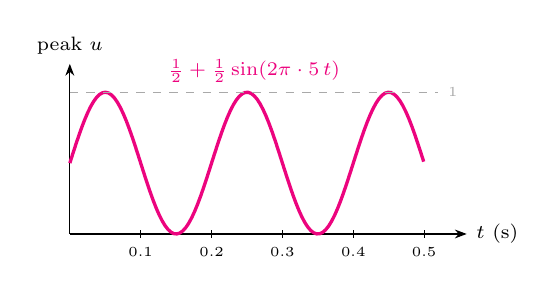
\begin{tikzpicture}[scale=0.9]
  \draw[-{Stealth[length=1.5mm]}] (0,0) -- (5.6,0) node[right,font=\scriptsize] {$t$ (s)};
  \draw[-{Stealth[length=1.5mm]}] (0,0) -- (0,2.4) node[above,font=\scriptsize] {peak $u$};
  \draw[RubineRed,very thick] plot[domain=0:0.5,samples=120] ({10*\x},{2*(0.5+0.5*sin(deg(2*pi*5*\x)))});
  \foreach \t in {0.1,0.2,0.3,0.4,0.5}{\draw ({10*\t},0.05) -- ({10*\t},-0.05) node[below,font=\tiny] {\t};}
  \draw[dashed,DarkGray] (0,2) -- (5.2,2) node[right,font=\tiny,text=DarkGray] {1};
  \node[font=\scriptsize,text=RubineRed] at (2.6,2.3) {$\tfrac12 + \tfrac12\sin(2\pi\cdot 5\,t)$};
\end{tikzpicture}
\vspace{2mm}

\small Peak velocity at the centreline versus time: period $1/f = 0.2$ s, maximum $1$ at $t = 0.05, 0.25, \ldots$, zero at $t = 0.15, 0.35, \ldots$ The flow never reverses; it pulses between still and full.
\end{column}
\begin{column}{0.48\textwidth}
\small At each instant the profile across the ends is the parabola of slide \ref{fr:space} with that peak; outside $|y| < d/2$ the ends are closed ($u = 0$), so the fluid outside the channel walls is driven only by what leaks around the target-point walls.
\vspace{1mm}

\small What to try (also in IB/02's README):
\begin{itemize}
  \item change \code{f} and watch the Womersley number $\alpha = \tfrac{d}{2}\sqrt{2\pi f\rho/\mu}$ change the profile from parabolic to plug-like;
  \item make the flow reverse with \code{sin(2*PI*f*t)} instead of \code{0.5 + 0.5*sin(...)};
  \item set \code{gcoef\_function\_1} to a traction condition ($a = 0$, $b = 1$, $g = 0$) and let the outlet find its own profile (slides \ref{fr:traction}, \ref{fr:open}).
\end{itemize}
\small The next two slides show the channel at a peak and at a trough of the pulse.
\end{column}
\end{columns}
\end{frame}

% 35
\begin{frame}{The pulsatile channel at a peak and at a trough}
\label{fr:ib02fig}
\begin{columns}[T,onlytextwidth]
\begin{column}{0.49\textwidth}
\centering
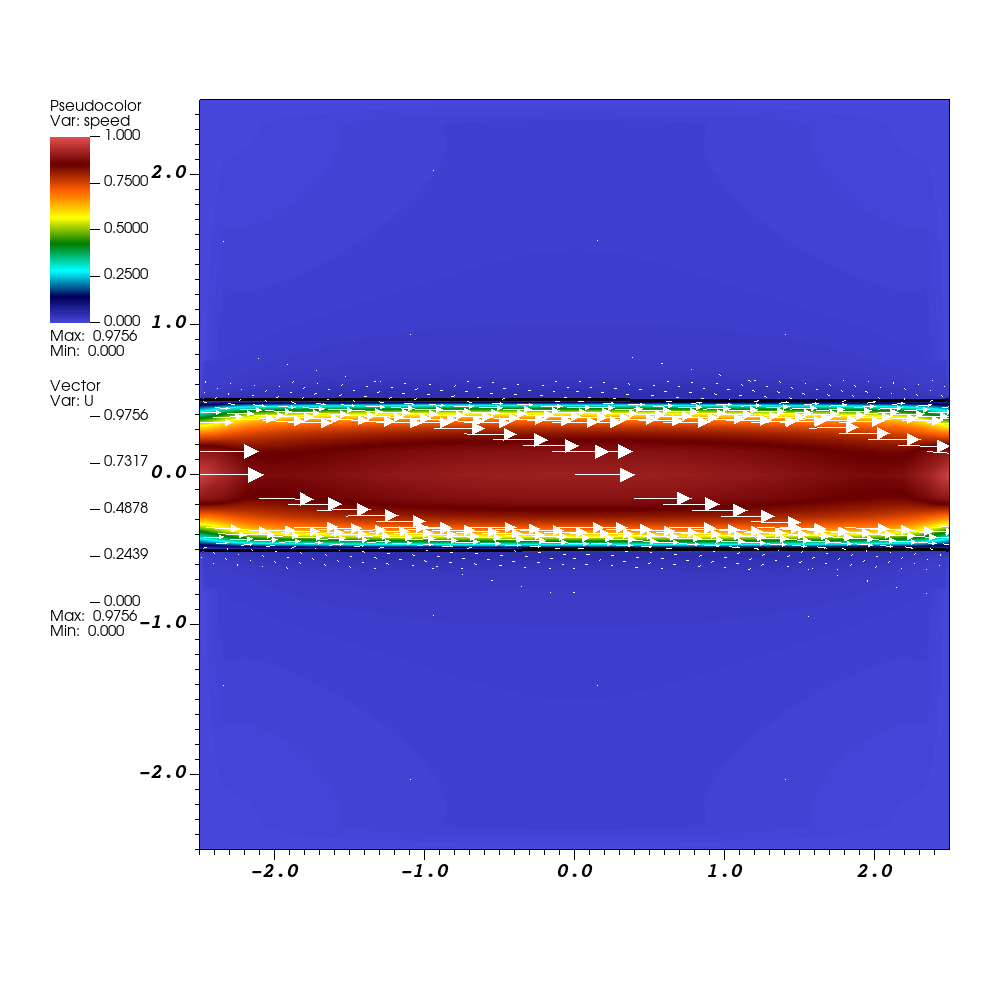
\includegraphics[height=0.5\textheight]{ch7-channel-peak-speed}\\
\scriptsize $t = 0.25$ s, a peak: the inlet factor is $1$.
\end{column}
\begin{column}{0.49\textwidth}
\centering
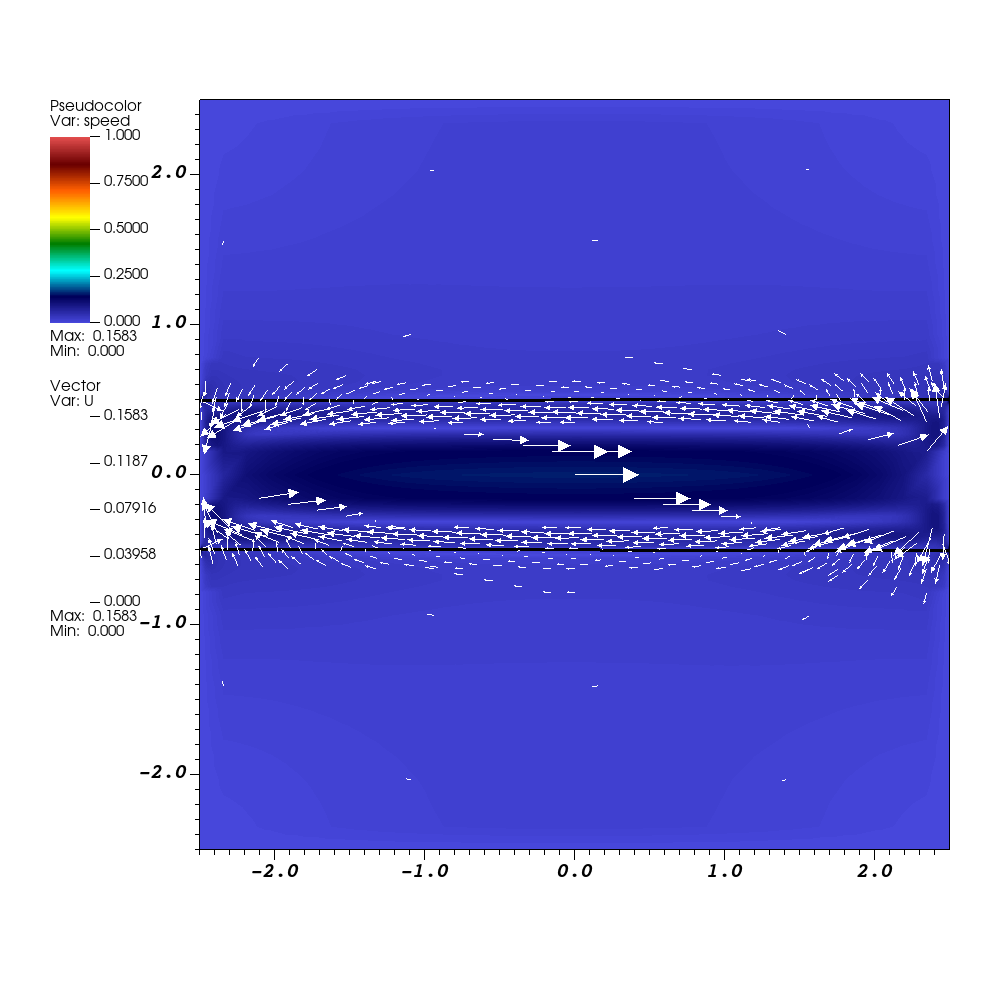
\includegraphics[height=0.5\textheight]{ch7-channel-trough-speed}\\
\scriptsize $t = 0.15$ s, a trough: the inlet factor is $0$.
\end{column}
\end{columns}
\vspace{1mm}
\footnotesize Speed from 0 (blue) to 1 (dark red) over the whole $5 \times 5$ box; the two channel walls are the black lines at $y = \pm 0.5$. At the peak the channel is full of fast fluid and the box outside the walls is still: the ends are closed there. At the trough the inlet has stopped but the fluid inside has not, and what remains moves fastest \emph{near the walls}, not at the centre.
\sourcecredit{IB/02 with its shipped input, run to 0.25 s (one and a quarter pulses), IBAMR 0.19.0; VisIt 3.5, \code{wsl/final/visit\_ch7b.sh}.}
\end{frame}

% 36
\begin{frame}{The channel inlet up close}
\label{fr:ib02fig2}
\begin{columns}[T,onlytextwidth]
\begin{column}{0.46\textwidth}
\centering
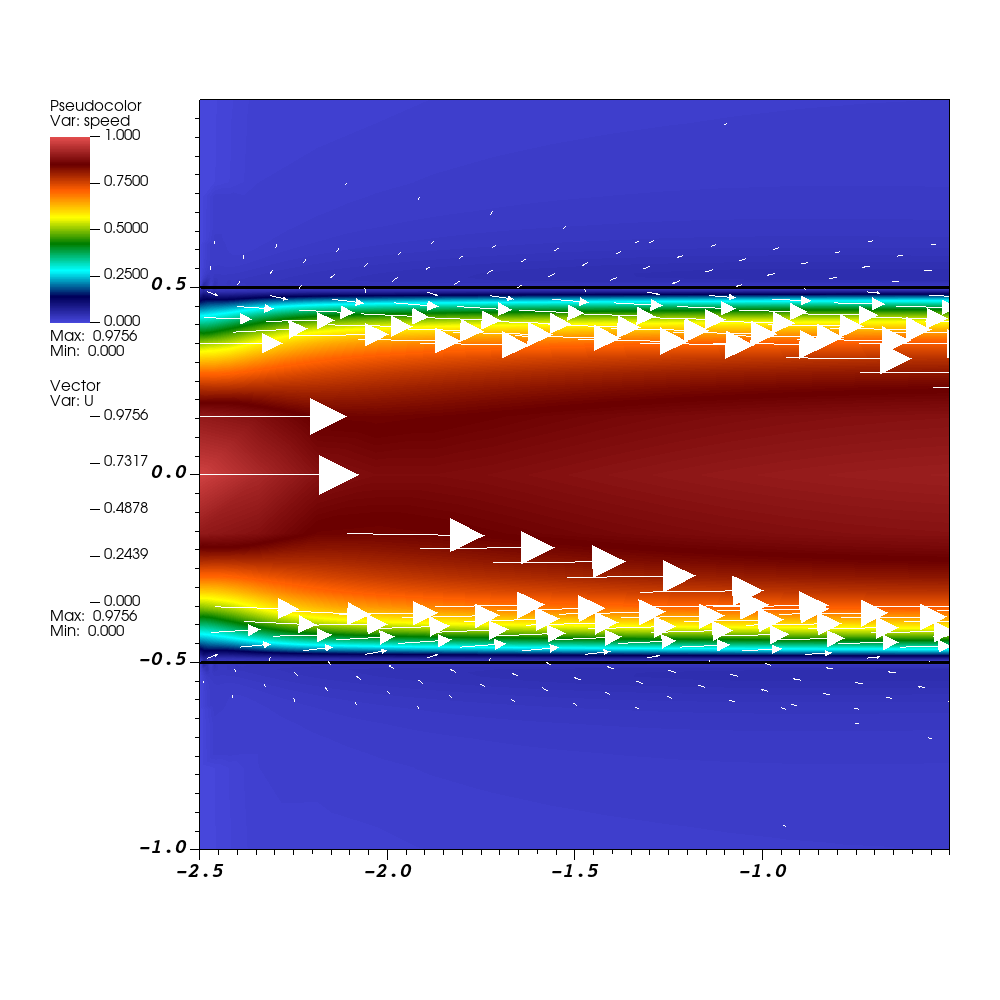
\includegraphics[height=0.58\textheight]{ch7-channel-inlet-speed}
\end{column}
\begin{column}{0.52\textwidth}
\footnotesize The left end of the box at the peak, $-2.5 \le x \le -0.5$. On the boundary ($x = -2.5$) the vectors trace the parabola of the expression: longest at $y = 0$, zero at $y = \pm 0.5$, and zero outside. A short way in, the profile is already flatter in the middle and steeper at the walls.
\vspace{1mm}

\footnotesize That is the \al{annular effect} of oscillatory flow: with $\nu = \mu/\rho = 0.1$ m$^2$/s and $f = 5$ Hz the Womersley number is $\alpha = 0.5\sqrt{2\pi\cdot5/0.1} \approx 8.9$, so the fluid in the core follows the pressure pulse as a plug while a thin Stokes layer at each wall lags it, and at the trough the layers are still moving when the core has stopped (previous slide). The inlet condition forces a parabola, which is the steady profile, not the oscillatory one; the flow adjusts within an entrance length.
\vspace{1mm}

\footnotesize A boundary condition prescribes the velocity \emph{on the side}; what the interior does with it is physics, and the first few cells in from the side are where the two meet.
\end{column}
\end{columns}
\sourcecredit{Same run; window $-2.5 \le x \le -0.5$, $-1 \le y \le 1$, $t = 0.25$ s.}
\end{frame}

% 37
\begin{frame}[fragile]{Example: a glycocalyx fibre in shear (IB/08): periodic sides, a floor and a lid}
\label{fr:ib08}
\begin{columns}[T,onlytextwidth]
\begin{column}{0.5\textwidth}
\footnotesize The 2020 lecture's \code{4-Example\_3DGlycocalyx}: a periodic array of fixed cylinders in shear flow. Periodic conditions in two directions, no slip on the bottom, a prescribed velocity at the top; the cylinder stands in the middle of the domain, coming out of the floor.
\begin{itemize}
  \item \code{periodic\_dimension = 1, 1, 0}: sides 0--3 are periodic, so their entries in the blocks are ignored (slide \ref{fr:periodic});
  \item side 4 (floor, $z$ lower): all components $0$;
  \item side 5 (lid, $z$ upper): $u = V\tanh 2t$, $v = w = 0$.
\end{itemize}
\footnotesize Only the $x$-block has a nonzero entry, on side 5. The course version wrote \code{"0.1*tanh(2*t)"}; the series version uses block constants so that \code{V} and the option \code{SHEAR\_START} (slide \ref{fr:ic2}) are set once at the top of the file.
\end{column}
\begin{column}{0.48\textwidth}
\begin{lstlisting}[style=inputtiny]
VelocityBcCoefs_0 {         // x-component
   V_LID = V
   SHEAR = SHEAR_START

   acoef_function_0 = "1.0"    // sides 0-3: periodic,
   acoef_function_1 = "1.0"    // these entries are
   acoef_function_2 = "1.0"    // ignored
   acoef_function_3 = "1.0"
   acoef_function_4 = "1.0"    // floor
   acoef_function_5 = "1.0"    // lid

   bcoef_function_0 = "0.0"
   ...
   bcoef_function_5 = "0.0"

   gcoef_function_0 = "0.0"
   ...
   gcoef_function_4 = "0.0"
   gcoef_function_5 = "V_LID*(SHEAR + (1 - SHEAR)*tanh(2*t))"
}
\end{lstlisting}
\end{column}
\end{columns}
\end{frame}

% 38
\begin{frame}[fragile]{Example: the 3D flow tank (IBFE/10): six sides, one constant}
\label{fr:ibfe10}
\begin{columns}[T,onlytextwidth]
\begin{column}{0.5\textwidth}
\begin{lstlisting}[style=inputtiny]
VelocityBcCoefs_0 {         // x-component
   U0 = U_FLOW   // copied here because the expressions
                 // can use only constants defined in their block
   acoef_function_0 = "1.0"
   ...
   acoef_function_5 = "1.0"

   bcoef_function_0 = "0.0"
   ...
   bcoef_function_5 = "0.0"

   gcoef_function_0 = "U0*tanh(2*t)"
   gcoef_function_1 = "U0*tanh(2*t)"
   gcoef_function_2 = "U0*tanh(2*t)"
   gcoef_function_3 = "U0*tanh(2*t)"
   gcoef_function_4 = "U0*tanh(2*t)"
   gcoef_function_5 = "U0*tanh(2*t)"
}
// VelocityBcCoefs_1 and _2: all a = 1, b = 0, g = 0
\end{lstlisting}
\end{column}
\begin{column}{0.48\textwidth}
\scriptsize The 3D version of the leaf's conditions: a thin elastic plate in a uniform stream $(U\tanh 2t, 0, 0)$ prescribed on all six faces of a $32 \times 16 \times 16$ tank. The tank is not periodic.
\begin{itemize}
  \item six sides means six entries per key in 3D; a 2D block has four. Copying a 2D block into a 3D input leaves sides 4 and 5 undefined, which is a warning and $a = b = g = 0$ on those sides (slide \ref{fr:err2}), not an error.
  \item the four faces where $u$ is tangential (2--5) are sliding walls again.
  \item the domain is longer in $x$ and the plate sits a quarter of the way in; the geometry block that does this is on slide \ref{fr:ex2}.
\end{itemize}
\scriptsize The IBFE method does not change the Eulerian boundary conditions at all: the blocks are read by the same \code{muParserRobinBcCoefs} and registered with the same Navier--Stokes integrator as in the IB examples.
\end{column}
\end{columns}
\end{frame}

% 39
\begin{frame}[fragile]{Scalar conditions: the temperature of IBFE/12}
\label{fr:scalar}
\begin{columns}[T,onlytextwidth]
\begin{column}{0.5\textwidth}
\begin{lstlisting}[style=inputtiny]
TemperatureBcCoefs {
   L = L

   acoef_function_0 = "1.0"
   acoef_function_1 = "1.0"
   acoef_function_2 = "1.0"
   acoef_function_3 = "1.0"

   bcoef_function_0 = "0.0"
   bcoef_function_1 = "0.0"
   bcoef_function_2 = "0.0"
   bcoef_function_3 = "0.0"

   gcoef_function_0 = "..."   // the initial T, so that the
   gcoef_function_1 = "..."   // boundary agrees with the
   gcoef_function_2 = "..."   // interior at t = 0
   gcoef_function_3 = "..."
}
\end{lstlisting}
\begin{lstlisting}[style=cpptiny]
// main.cpp of IBFE/12
T_bc_coef = std::make_unique<muParserRobinBcCoefs>("T_bc_coef",
    app_initializer->getComponentDatabase("TemperatureBcCoefs"), grid_geometry);
\end{lstlisting}
\end{column}
\begin{column}{0.48\textwidth}
\footnotesize An advected and diffused scalar (temperature, concentration) has a block of the same shape, under whatever name \code{main.cpp} asks for. Two differences from the velocity:
\begin{itemize}
  \item the coefficients are passed straight to the diffusion solver, which handles a general Robin condition, so $a$ and $b$ may \emph{both} be nonzero: $a\,T + b\,\partial T/\partial n = g$ with, say, $a = h$, $b = k$ is a convective (Newton cooling) condition. The upstream \code{adv\_diff} examples use Neumann ($b = 1$) sides;
  \item there is no ``traction'' meaning; $b = 1$, $g = 0$ is simply an insulated side, and $a = 1$ a prescribed value.
\end{itemize}
\footnotesize IBFE/12's domain is periodic in both directions, so its block is read but not used; it is there so that \code{periodic\_dimension = 0, 0} works without further edits. Chapter 15 covers the advection--diffusion solver itself.
\end{column}
\end{columns}
\end{frame}

% 40
\begin{frame}{Compatibility: net flux, the pressure level and \code{normalize\_pressure}}
\label{fr:compat}
\footnotesize Two consistency rules follow from incompressibility and from the pressure having no condition of its own.
\begin{enumerate}
  \item \al{Net flux.} If every side is a velocity condition or periodic, $\nabla\cdot\mathbf{u} = 0$ integrated over the box forces $\oint u_n\,dS = 0$. The solver cannot satisfy an inflow with closed walls; the projection will produce something, but not a solution of your problem. An open side (traction) removes the constraint: the flux through it is whatever balances the rest.
  \item \al{The pressure level.} With velocity conditions or periodic sides everywhere, the pressure is defined only up to a constant. \code{normalize\_pressure = TRUE} pins it by subtracting the mean every step; \code{FALSE} (the default) lets the solver's own null-space handling decide, and the level can drift without affecting the velocity. The IB examples in this series set it \code{TRUE}, the IBFE examples \code{FALSE}; both run. With at least one traction side the boundary fixes the level (slide \ref{fr:pressure}), and the mean must \emph{not} be removed: \code{normalize\_pressure = FALSE}, as in the upstream open-boundary examples (\code{IB/explicit/ex2}'s stabilized cylinder, \code{IIM/ex9}).
\end{enumerate}
\vspace{1mm}
\begin{punchbox}
\footnotesize A related key, \code{normalize\_velocity} (default \code{FALSE}), removes the mean velocity in fully periodic domains where it is otherwise undetermined (a periodic box with no walls can drift). Both are keys of the fluid integrator's block; the examples pass \code{NORMALIZE\_PRESSURE} from the top of the file.
\end{punchbox}
\end{frame}

% 41
\begin{frame}[fragile]{Open boundaries in practice: the upstream cylinder (IB/explicit/ex2)}
\label{fr:open}
\begin{columns}[T,onlytextwidth]
\begin{column}{0.52\textwidth}
\begin{lstlisting}[style=inputtiny]
NORMALIZE_PRESSURE  = FALSE   // an open side fixes the level

VelocityBcCoefs_0 {           // x-component
   t_half = 0.5
   tau = 0.125

   acoef_function_0 = "1.0"   // left: velocity (inflow)
   acoef_function_1 = "0.0"   // right: traction (open)
   acoef_function_2 = "0.0"   // bottom: traction
   acoef_function_3 = "0.0"   // top: traction

   bcoef_function_0 = "0.0"
   bcoef_function_1 = "1.0"
   bcoef_function_2 = "1.0"
   bcoef_function_3 = "1.0"

   gcoef_function_0 = "(tanh((t-t_half)/tau)+tanh(t_half/tau))/(1+tanh(t_half/tau))"
   gcoef_function_1 = "0.0"
   gcoef_function_2 = "0.0"
   gcoef_function_3 = "0.0"
}
\end{lstlisting}
\end{column}
\begin{column}{0.46\textwidth}
\footnotesize \code{examples/IB/explicit/ex2/}\allowbreak\code{input2d.cylinder\_stabilized} in the 0.19.0 tree: flow past a cylinder with an inflow on the left and an \al{open right side}. The $x$-block:
\begin{itemize}
  \item side 0: $u = $ a smooth ramp from $0$ to $1$ centred at $t = 0.5$ with width $0.125$ (another way to write the start-up of slide \ref{fr:time});
  \item side 1: $(a, b) = (0, 1)$, $g = 0$: zero normal stress, so $p \approx 0$ there (slide \ref{fr:pressure}); the outlet velocity is whatever the interior produces;
  \item sides 2 and 3: $(a, b) = (0, 1)$, $g = 0$ on $u$, which is \emph{tangential} there: zero shear stress along the top and bottom.
\end{itemize}
\footnotesize The $y$-block on the next slide completes the picture.
\end{column}
\end{columns}
\end{frame}

% 42b
\begin{frame}[fragile]{The upstream cylinder: free-slip walls and a nudge to start shedding}
\label{fr:open2}
\begin{columns}[T,onlytextwidth]
\begin{column}{0.52\textwidth}
\begin{lstlisting}[style=inputtiny]
VelocityBcCoefs_1 {           // y-component
   acoef_function_0 = "1.0"   // left: velocity
   acoef_function_1 = "0.0"   // right: traction
   acoef_function_2 = "1.0"   // bottom: velocity
   acoef_function_3 = "1.0"   // top: velocity

   bcoef_function_0 = "0.0"
   bcoef_function_1 = "1.0"
   bcoef_function_2 = "0.0"
   bcoef_function_3 = "0.0"

   gcoef_function_0 = "cos(pi*X_1/16.0)*exp(-0.5*t)"
   gcoef_function_1 = "0.0"
   gcoef_function_2 = "0.0"
   gcoef_function_3 = "0.0"
}
\end{lstlisting}
\end{column}
\begin{column}{0.46\textwidth}
\scriptsize
\begin{itemize}
  \item side 0: $v = \cos(\pi y/16)\,e^{-t/2}$, a small transverse velocity that dies away in a few seconds: a \al{nudge} that breaks the symmetry so that vortex shedding starts without waiting for round-off to do it;
  \item side 1: traction with $g = 0$ on $v$ too, so the outlet is open in \emph{both} components: zero normal stress and zero shear, the fully open outlet of slide \ref{fr:traction};
  \item sides 2 and 3: $v = 0$, a velocity condition on the \emph{normal} component (no flow through), combined with the zero shear on $u$ from the previous slide: \al{free-slip walls}, which confine the flow without boundary layers.
\end{itemize}
\scriptsize The wake leaves through the right side at whatever velocity it has; nothing squeezes it back to uniform. The price is possible \al{backflow} at the outlet, which the next slide handles. \code{NORMALIZE\_PRESSURE = FALSE} because side 1 fixes the pressure level (slide \ref{fr:compat}).
\end{column}
\end{columns}
\end{frame}

% 42
\begin{frame}[fragile]{Backflow at an open side: the open-boundary stabilizer}
\label{fr:stab}
\small An open outlet lets fluid come \emph{in} wherever the wake's velocity points inward, and an open inlet lets it leave. Either can feed an instability. IBAMR's remedy is \code{StaggeredStokesOpenBoundaryStabilizer}, a body force applied in a layer next to the side that pushes the offending velocity back toward zero. From the source:
\begin{lstlisting}[style=cpptiny]
if ((d_inflow_bdry[location_index] && U * n > 0.0) || (d_outflow_bdry[location_index] && U * n < 0.0))
    (*F_data)(i_s) = smooth_kernel((x - x_bdry) / d_width[location_index]) * kappa * (0.0 - U);
\end{lstlisting}
\begin{columns}[T,onlytextwidth]
\begin{column}{0.46\textwidth}
\footnotesize In the input file (\code{IB/explicit/ex2}'s stabilized cylinder; \code{IIM/ex9} does the same for sides 4 and 5 with \code{"INFLOW"} on 4):
\begin{lstlisting}[style=inputtiny]
BoundaryStabilization {
   stabilization_type_1 = "OUTFLOW"
   width_1 = 4.0*DX_FINEST
}
\end{lstlisting}
\footnotesize Keys \code{stabilization\_type\_s} (\code{"INFLOW"}, \code{"OUTFLOW"} or \code{"NONE"}) and \code{width\_s} per side; four fine cells is the usual width.
\end{column}
\begin{column}{0.52\textwidth}
\footnotesize It is registered in \code{main.cpp}, not automatically; \code{IB/explicit/ex2} does so only when the block exists and the solver is staggered:
\begin{lstlisting}[style=cpptiny]
if (solver_type == "STAGGERED" && input_db->keyExists("BoundaryStabilization"))
    time_integrator->registerBodyForceFunction(
        new StaggeredStokesOpenBoundaryStabilizer(
            "BoundaryStabilization",
            app_initializer->getComponentDatabase("BoundaryStabilization"),
            navier_stokes_integrator, grid_geometry));
\end{lstlisting}
\footnotesize The examples in this series do not register it (they have no open sides). Chapter 15 reads \code{IB/explicit/ex2} in full.
\end{column}
\end{columns}
\end{frame}

% 43
\begin{frame}[fragile]{Periodic sides: \code{periodic\_dimension} overrides everything}
\label{fr:periodic}
\begin{columns}[T,onlytextwidth]
\begin{column}{0.5\textwidth}
\begin{lstlisting}[style=inputtiny]
CartesianGeometry {
   domain_boxes = [ (0,0) , (N - 1,N - 1) ]
   x_lo = -0.5*L, -0.5*L   // lower end of computational domain.
   x_up =  0.5*L,  0.5*L   // upper end of computational domain.
   periodic_dimension = 1, 1
}
\end{lstlisting}
\small \code{periodic\_dimension} turns on periodic boundary conditions, one flag per direction: $1$ is on, $0$ is off. A periodic direction identifies its two sides: what leaves through side 1 enters through side 0. The block above (the 2013--2020 slide) makes the whole box periodic; IB/08 uses \code{1, 1, 0}; IBFE/12 uses \code{1, 1}; the other examples in this series use all zeros and the \code{VelocityBcCoefs} blocks.
\end{column}
\begin{column}{0.48\textwidth}
\small What it means in practice:
\begin{itemize}
  \item on a periodic direction's two sides the \code{VelocityBcCoefs} entries are \al{ignored, silently}. Tested: IB/03 with \code{periodic\_dimension = 1, 0} and the inflow still written on sides 0 and 1 runs without a warning, and no inflow happens (slide \ref{fr:err2});
  \item the Lagrangian points cross a periodic side and re-enter on the other (the \code{LDataManager} applies the periodic shift); a structure may straddle it.
\end{itemize}
\small More consequences on the next slide.
\end{column}
\end{columns}
\end{frame}

% 44
\begin{frame}{Periodic sides: consequences}
\label{fr:periodic2}
\small
\begin{itemize}
  \item In a fully periodic box there are no walls to hold the fluid still, so the mean velocity can drift (\code{normalize\_velocity}, slide \ref{fr:compat}), and nothing can be ``in flow'' unless a body force or a moving structure drives it. IBFE/12 (periodic both ways) moves its scalar with a prescribed velocity field, not with a boundary condition.
  \item The periodic length is \code{x\_up - x\_lo}, which must be larger than the structure plus its wake if the images are not to interact. IB/08 \emph{wants} the interaction: the fibre is one of an infinite array, $1/8$ m apart.
  \item A direction can be periodic while the others carry boundary conditions: IB/08 is periodic in $x$ and $y$ and has a floor and a lid in $z$. The entries for sides 0--3 must still be present in the blocks (or the missing-key warning appears), and they may say anything.
  \item Periodic in the \emph{flow} direction turns an inflow--outflow problem into a driven one: the leaf with \code{periodic\_dimension = 1, 0} sees its own wake arrive from upstream, and the only thing moving the fluid is the sliding top and bottom (the tested case of slide \ref{fr:err2}).
  \item Refinement patches may cross a periodic side; the gridding algorithm handles the wrap, and VisIt draws the levels in the box as usual.
\end{itemize}
\end{frame}

% 45
\begin{frame}[fragile]{Initial conditions}
\label{fr:ic}
\begin{columns}[T,onlytextwidth]
\begin{column}{0.5\textwidth}
\begin{lstlisting}[style=inputtiny]
VelocityInitialConditions {        // IB/03: at rest
   function_0 = "0.0"
   function_1 = "0.0"
}

VelocityInitialConditions {        // IB/08: an option
   SHEAR = SHEAR_START
   V0 = V
   L0 = L
   function_0 = "SHEAR*V0*(X_2 + 0.5*L0)/L0"
   function_1 = "0.0"
   function_2 = "0.0"
}
\end{lstlisting}
\footnotesize \code{main.cpp} registers the block if it exists (\code{keyExists("VelocityInitialConditions")}), likewise \code{PressureInitialConditions} with its single \code{function}; the examples in this series have only the velocity block.
\end{column}
\begin{column}{0.48\textwidth}
\small \code{function\_d} is the $d$-th velocity component at $t = 0$ as an expression in \code{X\_0}, \code{X\_1}, \code{X\_2} (and \code{t}, which is $0$), with the same parser and the same block-constant rule as the boundary blocks.
\begin{itemize}
  \item \al{Start from rest} unless you have a reason not to: it is consistent with any ramped boundary condition, and chapter 16's first rule for an unstable run is ``start from zero velocity''.
  \item The initial velocity should agree with the boundary condition at $t = 0$; a mismatch is a (one-step) impulsive start.
\end{itemize}
\end{column}
\end{columns}
\end{frame}

% 46
\begin{frame}{Initial conditions, continued: a non-trivial start}
\label{fr:ic2}
\small
\begin{itemize}
  \item IB/08's option: with \code{SHEAR\_START = 1} the fluid starts in the linear shear profile that the lid would produce, $u = V(z + L/2)/L$, and the lid moves at $V$ from the first step (slide \ref{fr:time}); the fibre feels the flow at once instead of after the viscous start-up, which takes $0.2$ s or more to reach the floor (the README has the 1D solution and the measured profiles).
  \item The two must match: the initial profile has $u = V$ at the lid and $0$ at the floor, which is exactly what the boundary blocks say at $t = 0$ with \code{SHEAR = 1}. Change one and not the other and the first step is impulsive.
  \item An initial condition that does not satisfy $\nabla\cdot\mathbf{u} = 0$ is projected at the first step; what you see in frame 0 is what you wrote, what you see in frame 1 is the divergence-free part of it.
  \item The pressure initial condition is used only for the first output frame (slide \ref{fr:ex0}); \code{navier\_stokes/ex0} sets it because the exact solution is known and the error is measured from frame 0.
  \item A structure's initial state is the \code{.vertex} file (chapter 6), not an expression; the fluid and the structure start independently, and a structure that starts stretched or bent releases its energy into fluid that is at rest.
\end{itemize}
\end{frame}

% 47
\begin{frame}{Part II: changing the size of the domain, making it rectangular, and the grid}
\label{fr:part2}
\Large\color{NavyBlue} Part II: the domain and its grid\par
\vspace{3mm}
\normalsize\color{black}
The \code{CartesianGeometry} block; levels, refinement ratio and cell counts; two worked examples (a tall thin box, a long tank); the divisibility rules; patch sizes; tagging and regridding; keeping the structure off the edge; a first guess at $\Delta t$; output intervals and disk space; checking before a long run.
\vspace{3mm}

\small This is the 2017 ``Using different domain dimensions'' deck and Part II of the 2020 Lecture 4, with the 2015 lecture's cautions on grid refinement.
\end{frame}

% 48
\begin{frame}[fragile]{\code{CartesianGeometry}: the index box and the physical box}
\label{fr:geom}
\begin{columns}[T,onlytextwidth]
\begin{column}{0.5\textwidth}
\begin{lstlisting}[style=inputtiny]
CartesianGeometry {
   domain_boxes = [ (0,0,0) , (N/8 - 1,N/8 - 1,N - 1) ]
   x_lo = -L/16, -L/16, -L/2   // lower end of computational domain.
   x_up =  L/16,  L/16,  L/2   // upper end of computational domain.
   periodic_dimension = 1, 1, 0
}
\end{lstlisting}
\footnotesize (IB/08; a 2D block has pairs instead of triples.)
\begin{itemize}
  \item \code{domain\_boxes}: the cells of the \al{coarsest} level, as an index box from $(0,0,0)$ to $(M_x - 1, M_y - 1, M_z - 1)$ where $M_d$ is the number of coarsest cells in direction $d$. A list, because SAMRAI allows several boxes; IBAMR uses one.
  \item \code{x\_lo}, \code{x\_up}: the physical corners, in metres (or whatever unit the rest of the file uses). The lower corner sets $x_{\min}, y_{\min}, (z_{\min})$ and the upper one the maxima.
  \item \code{periodic\_dimension}: slide \ref{fr:periodic}.
\end{itemize}
\end{column}
\begin{column}{0.48\textwidth}
\footnotesize The cell size on the coarsest level is $(x_{\mathrm{up}} - x_{\mathrm{lo}})_d / M_d$ in each direction, and on level $\ell$ it is that divided by the refinement ratio $\ell$ times. Nothing forces the three cell sizes to be equal, but the IB kernels and every example assume \al{square (cubic) cells}: keep the physical lengths in the same proportion as the cell counts. IB/08: $\frac{1}{8} : \frac{1}{8} : 1$ and $4 : 4 : 32$. IBFE/10: $32 : 16 : 16$ and $32 : 16 : 16$.
\vspace{1mm}

\footnotesize The coarsest box is what you type; the finer levels are made by the gridding algorithm (next slide) and never typed. So \al{``changing the size of the domain''} means changing \code{x\_lo}/\code{x\_up} \emph{and} \code{domain\_boxes} together, or the cells change shape.
\end{column}
\end{columns}
\end{frame}

% 49
\begin{frame}[fragile]{Levels, refinement ratio, \code{N} and \code{NFINEST}}
\label{fr:levels}
\begin{columns}[T,onlytextwidth]
\begin{column}{0.5\textwidth}
\begin{lstlisting}[style=inputtiny]
MAX_LEVELS = 3                            // maximum number of levels
REF_RATIO  = 4                            // refinement ratio between levels
N = 32                                    // cells on the coarsest level
NFINEST = (REF_RATIO^(MAX_LEVELS - 1))*N  // cells on the finest level
DX = (1.0*L)/NFINEST                      // finest mesh width (m)

GriddingAlgorithm {
   max_levels = MAX_LEVELS
   ratio_to_coarser {
      level_1 = REF_RATIO,REF_RATIO
      level_2 = REF_RATIO,REF_RATIO
      ...
   }
   ...
}
\end{lstlisting}
\end{column}
\begin{column}{0.48\textwidth}
\small IBAMR refines the grid near the structure (and, optionally, where the vorticity is large). \code{MAX\_LEVELS} is the number of levels including the coarsest; \code{REF\_RATIO} the ratio of cell counts between a level and the next coarser one, the same in every direction.
\[
  \mathrm{NFINEST} = \mathrm{REF\_RATIO}^{\,\mathrm{MAX\_LEVELS}-1}\times N .
\]
\small \code{DX} is the finest mesh width; it is what the structure's point spacing (chapter 6, $\Delta s \approx \Delta x/2$) and the $\Delta t$ guess (slide \ref{fr:dt}) refer to. The \code{ratio\_to\_coarser} list must have an entry for every level above the coarsest; extra entries (the UNC inputs list five) are harmless.
\end{column}
\end{columns}
\end{frame}

% 50
\begin{frame}{Levels and ratios: the 2015 example and what the examples use}
\label{fr:levels2}
\small The 2015 lecture's example: a $1 \times 1$ domain with $N = 8$, four levels and ratio 4 gives $8 \to 32 \to 128 \to 512$: the finest grid would be $512 \times 512$ \emph{if it covered the whole box}; it covers only the tagged region. ``Setting \code{MAX\_LEVELS} to 4 is a good default; \code{REF\_RATIO = 4} is a rather strict refinement ratio.''
\vspace{1mm}

\scriptsize
\begin{tabular}{@{}L{0.3\textwidth}cccL{0.3\textwidth}@{}}
\toprule
example & \code{N} & levels & finest & note\\
\midrule
IB/01, 06, 07 & 8 & 4 & 512 & the 2015 recipe\\
IB/02, 03 & 32 & 3 & 512 & same finest grid, one level fewer\\
IB/04 (moving cylinders) & 16 & 4 & 1024 & the finest grid in the series\\
IB/08 (3D) & 32 & 3 & $64 \times 64 \times 512$ & \code{N} counts the long direction\\
IBFE/01, 05, 06, 08, 12 & 32 & 2 & 128 & two levels: the finite-element mesh carries the resolution\\
IBFE/10 (3D) & 16 & 3 & $512 \times 256 \times 256$ & \code{N} counts the short directions\\
\bottomrule
\end{tabular}

\vspace{2mm}

\small A ratio of 2 with more levels gives a gentler nesting and more regrid work; a ratio of 4 with fewer levels is what every example here uses. The number of levels is the real cost lever: each level is another full set of patches, ghost cells and solver sweeps.
\end{frame}

% 51
\begin{frame}{Worked example 1: a tall thin box for the glycocalyx (2017, 2020)}
\label{fr:ex1}
\small ``Making the lengths of the domain different sizes.'' The changes are made in the input file, and you have to think the refinement levels through so that they make sense. The target: a box of physical size $\frac18 \times \frac18 \times 1$ with a finest grid of $64 \times 64 \times 512$.
\begin{enumerate}
  \item Let \code{NFINEST} be the number of finest cells in the \al{longest} direction: $512$. In the two short directions there are $\mathrm{NFINEST}/8 = 64$.
  \item Three levels, because the grid is so small in two directions; ratio 4. Then the coarsest level in the long direction has $N = 512 \times (\tfrac14)^{3-1} = 32$ cells, and in the short directions $N/8 = 4$.
  \item The cells are cubes: $1/512$ in every direction, because $\frac18 / 64 = 1/512$ too.
  \item The index box runs from $0$ to $M - 1$ in each direction, $M$ being the coarsest count: from $(0,0,0)$ to $(3, 3, 31)$, written with the constants as on the next slide.
  \item The physical box is centred: from $(-\tfrac1{16}, -\tfrac1{16}, -\tfrac12)$ to $(\tfrac1{16}, \tfrac1{16}, \tfrac12)$, with $L = 1$.
\end{enumerate}
\vspace{1mm}
\begin{punchbox}
\small \al{Four cells across the coarsest level} is as low as one should go (slide \ref{fr:rules}). The 2020 summary: ``make sure you don't have a coarsest level of size 1 (or even 2) in any dimension.''
\end{punchbox}
\end{frame}

% 52
\begin{frame}[fragile]{Worked example 1: the input lines, and the levels in a picture}
\label{fr:ex1b}
\begin{columns}[T,onlytextwidth]
\begin{column}{0.56\textwidth}
\begin{lstlisting}[style=inputtiny]
MAX_LEVELS = 3        // three levels: the grid is small in two directions
REF_RATIO  = 4
N = 32                // coarsest cells in the LONGEST direction
NFINEST = (REF_RATIO^(MAX_LEVELS - 1))*N   // 512 in the longest direction

CartesianGeometry {
   domain_boxes = [ (0,0,0) , (N/8 - 1,N/8 - 1,N - 1) ]
   x_lo = -L/16, -L/16, -L/2
   x_up =  L/16,  L/16,  L/2
   periodic_dimension = 1, 1, 0
}
\end{lstlisting}
\footnotesize In IB/08 as shipped, with its fibre of 13,600 target points standing on the floor; the finest level covers the fibre and a margin, the coarsest the whole column.
\end{column}
\begin{column}{0.42\textwidth}
\centering
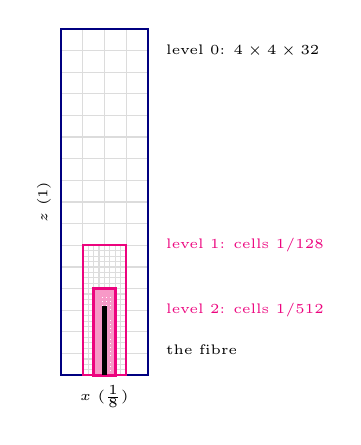
\begin{tikzpicture}[scale=0.55]
  \draw[step=0.5,LightGray!80] (0,0) grid (2,8);
  \draw[NavyBlue,thick] (0,0) rectangle (2,8);
  \draw[step=0.125,DarkGray!40] (0.5,0) grid (1.5,3);
  \draw[RubineRed,thick] (0.5,0) rectangle (1.5,3);
  \draw[step=0.03125,RubineRed!40] (0.75,0) grid (1.25,2);
  \draw[RubineRed,very thick] (0.75,0) rectangle (1.25,2);
  \draw[black,line width=1.5pt] (1,0) -- (1,1.6);
  \node[font=\tiny,anchor=west] at (2.2,7.5) {level 0: $4\times4\times32$};
  \node[font=\tiny,anchor=west,text=RubineRed] at (2.2,3.0) {level 1: cells $1/128$};
  \node[font=\tiny,anchor=west,text=RubineRed] at (2.2,1.5) {level 2: cells $1/512$};
  \node[font=\tiny,anchor=west] at (2.2,0.6) {the fibre};
  \node[font=\tiny] at (1,-0.5) {$x$ ($\tfrac18$)};
  \node[font=\tiny,rotate=90] at (-0.4,4) {$z$ ($1$)};
\end{tikzpicture}
\vspace{1mm}

\scriptsize A $y$-slice: the coarsest level fills the column, the finer levels nest around the fibre (schematic; the real patches are chosen by the gridding algorithm, slide \ref{fr:patches}).
\end{column}
\end{columns}
\end{frame}

% 53
\begin{frame}[fragile]{Worked example 2: a long tank with the plate a quarter of the way in (IBFE/10)}
\label{fr:ex2}
\begin{columns}[T,onlytextwidth]
\begin{column}{0.52\textwidth}
\begin{lstlisting}[style=inputtiny]
L = 16.0              // width of computational domain
MAX_LEVELS = 3
REF_RATIO  = 4
N = 16                // coarsest cells across (y and z)
NFINEST = (REF_RATIO^(MAX_LEVELS - 1))*N   // 256 across
DX  = L/NFINEST       // 1/16

CartesianGeometry {
   domain_boxes = [ (0,0,0),(2*N - 1,N - 1,N - 1) ]
   x_lo = -0.5*L,-0.5*L,-0.5*L
   x_up =  1.5*L, 0.5*L, 0.5*L
   periodic_dimension = 0,0,0
}
\end{lstlisting}
\end{column}
\begin{column}{0.46\textwidth}
\footnotesize Here the \al{short} directions carry \code{N}, and the long one is \code{2*N}: a $32 \times 16 \times 16$ coarsest grid for a $32 \times 16 \times 16$ tank, cubes of side 1 on level 0 and $1/16$ on level 2.
\begin{itemize}
  \item \code{x\_lo} and \code{x\_up} need not be symmetric: $x$ runs from $-8$ to $24$, so the plate at the origin sits $8$ units from the inlet and $24$ from the outlet, where its wake has room.
  \item \code{NFINEST} is a name, not a rule: it counts the finest cells \emph{across} here and \emph{along} in IB/08. What matters is that \code{DX} is the same in every direction.
  \item the three cell counts $32, 16, 16$ are all multiples of $\mathrm{REF\_RATIO}^{\,2} = 16$, so each level's cells line up with the next (slide \ref{fr:rules}).
\end{itemize}
\end{column}
\end{columns}
\end{frame}

% 54
\begin{frame}{The rules: divisibility, minimum sizes, square cells}
\label{fr:rules}
\footnotesize From the 2020 summary slide, with the reasons:
\begin{enumerate}
  \item \al{Each coarsest cell count must be a whole number}, and the finest count in each direction must be divisible by $\mathrm{REF\_RATIO}^{\,\mathrm{MAX\_LEVELS}-1}$: the levels are built by refining whole coarse cells, so the finest grid is the coarsest times a power of the ratio, in every direction. Decide the finest resolution you want, divide down, and round the coarsest count \emph{up} to a whole number.
  \item \al{No coarsest level of size 1, or even 2, in any direction.} The coarsest level must hold the smallest patch (slide \ref{fr:patches}) and SAMRAI's ghost-cell layers; the multigrid solvers want something to coarsen; and the refined region cannot be placed with any accuracy when the coarse cells are as big as the structure. Four is a practical minimum (IB/08); eight is comfortable.
  \item \al{Keep the cells square}: physical lengths in the same ratio as cell counts (slide \ref{fr:geom}).
  \item \al{The patch sizes must fit}: the smallest patch must divide the coarsest box in each direction, and the largest patch must be at least the smallest (slide \ref{fr:patches}).
\end{enumerate}
\vspace{1mm}
\begin{punchbox}
\footnotesize A quick check for a new domain: write $M_x, M_y, M_z$ (coarsest counts) and $\mathrm{NFINEST}_d = M_d\,r^{\,\ell-1}$; confirm $(x_{\mathrm{up}} - x_{\mathrm{lo}})_d / \mathrm{NFINEST}_d$ is the same number for every $d$; confirm each $M_d \ge 4$ and divisible by the smallest patch size.
\end{punchbox}
\end{frame}

% 55
\begin{frame}[fragile]{Patch sizes: \code{largest\_patch\_size} and \code{smallest\_patch\_size}}
\label{fr:patches}
\begin{columns}[T,onlytextwidth]
\begin{column}{0.5\textwidth}
\begin{lstlisting}[style=inputtiny]
   largest_patch_size {
      level_0 = NFINEST/8, NFINEST/8, NFINEST/8
      // NOTE: all finer levels will use same values as level_0...
   }
   smallest_patch_size {
      level_0 = 4, 4, 4
      // NOTE: all finer levels will use same values as level_0...
   }
\end{lstlisting}
\footnotesize (IB/08.) The 2020 heuristic: ``the largest patch size should be a cube of the finest grid that fills the domain in the shortest direction(s); the smallest patch size should be a cube of the coarsest grid that fills the domain in the shortest directions'': $64^3$ and $4^3$ here.
\vspace{1mm}

\footnotesize A level is made of rectangular \al{patches}; these keys bound their size in cells. The limits are per level but, with only \code{level\_0} given, apply to all levels.
\end{column}
\begin{column}{0.48\textwidth}
\scriptsize
\begin{itemize}
  \item smaller patches: better load balance across processes, more boundary and ghost-cell overhead;
  \item larger patches: fewer, bigger blocks; fine for one process, poor for sixteen.
\end{itemize}
\scriptsize The examples disagree, which shows these are heuristics, not rules:
\vspace{1mm}

\scriptsize
\begin{tabular}{@{}L{0.4\textwidth}L{0.28\textwidth}L{0.2\textwidth}@{}}
\toprule
example & largest & smallest\\
\midrule
IB/01, 02, 04, 06, 07 & \code{NFINEST, NFINEST} & \code{8, 8}\\
IB/03 & \code{NFINEST, NFINEST} & \code{32, 32}\\
IB/08 & \code{NFINEST/8} cubed & \code{4, 4, 4}\\
IBFE/01, 05, 06, 08, 12 & \code{512, 512} & \code{8, 8}\\
IBFE/10 & \code{256, 256, 256} & \code{8, 8, 8}\\
\bottomrule
\end{tabular}

\vspace{1mm}

\scriptsize The smallest patch must divide the coarsest box: $32 \times 32$ on IB/03's $32^2$ coarsest grid is one patch; $4^3$ on $4 \times 4 \times 32$ gives eight. A largest patch bigger than the grid (the IBFE $512^2$ on a $128^2$ finest grid) is simply no limit.
\end{column}
\end{columns}
\end{frame}

% 56
\begin{frame}[fragile]{The rest of the gridding block: efficiency and the tagging method}
\label{fr:gridding}
\begin{columns}[T,onlytextwidth]
\begin{column}{0.5\textwidth}
\begin{lstlisting}[style=inputtiny]
GriddingAlgorithm {
   ...
   efficiency_tolerance = 0.85e0  // min % of tag cells in new patch level
   combine_efficiency   = 0.85e0  // chop box if sum of volumes of smaller
                                  // boxes < efficiency * vol of large box
}

StandardTagAndInitialize {
   tagging_method = "GRADIENT_DETECTOR"
}
\end{lstlisting}
\end{column}
\begin{column}{0.48\textwidth}
\small
\begin{itemize}
  \item \code{efficiency\_tolerance}: a new patch must be at least this fraction tagged cells (0.85 in the IB examples, 0.80 in IBFE/10); lower values give fewer, fatter patches with more untagged cells refined.
  \item \code{combine\_efficiency}: when to split a box into smaller ones rather than keep one with untagged corners.
  \item \code{tagging\_method = "GRADIENT\_DETECTOR"}: the integrator tags cells itself; for IB that means the cells that contain Lagrangian points (plus the vorticity test on slide \ref{fr:vort}, if on). The name is SAMRAI's; IBAMR's integrators implement the ``gradient detector'' call-back with their own criteria.
\end{itemize}
\end{column}
\end{columns}
\end{frame}

% 57
\begin{frame}[fragile]{The rest of the gridding block: the tag buffer and when to regrid}
\label{fr:gridding2}
\begin{columns}[T,onlytextwidth]
\begin{column}{0.5\textwidth}
\begin{lstlisting}[style=inputtiny]
IBHierarchyIntegrator {
   ...
   regrid_cfl_interval = REGRID_CFL_INTERVAL   // 0.5 in the examples
   tag_buffer          = TAG_BUFFER            // 1 in the examples
}
\end{lstlisting}
\begin{lstlisting}[style=tiny]
IBHierarchyIntegrator::initializePatchHierarchy(): tag_buffer = 1 3
\end{lstlisting}
\scriptsize (the log line that confirms the setting; the second number is the buffer for the next level, computed from the first)
\end{column}
\begin{column}{0.48\textwidth}
\footnotesize
\begin{itemize}
  \item \code{tag\_buffer}: how many extra cells around a tagged cell are refined with it, per level. The buffer is what lets the structure move between regrids without leaving the fine level.
  \item \code{regrid\_cfl\_interval}: regrid whenever any Lagrangian point could have moved this many mesh widths since the last regrid (the IB integrators); the alternative key \code{regrid\_interval} regrids every so many steps. Regridding is expensive (new patches, data transfer, solver set-up), so $0.5$ with a buffer of $1$ is the usual balance.
  \item A structure that moves fast needs a larger buffer or a smaller interval; the symptom of too little is a point that steps off the finest level, which the log reports and the run may not survive (chapter 16).
\end{itemize}
\end{column}
\end{columns}
\end{frame}

% 58
\begin{frame}[fragile]{Refining on vorticity (the 2015 cautions)}
\label{fr:vort}
\begin{columns}[T,onlytextwidth]
\begin{column}{0.46\textwidth}
\begin{lstlisting}[style=inputtiny]
   using_vorticity_tagging = TRUE
   vorticity_abs_thresh = 0.25
   // or, instead of the absolute threshold:
   vorticity_rel_thresh = 0.25
\end{lstlisting}
\footnotesize (Keys of the fluid integrator's block, \code{INSStaggeredHierarchyIntegrator}; the examples set \code{VORTICITY\_TAGGING = FALSE} at the top of the file and pass it in.)
\vspace{1mm}

\footnotesize ``You can also set vortices for local refinement. If you set this too small, you will tag the whole domain for refinement! If it is too big, you won't resolve the vortex wake.''
\end{column}
\begin{column}{0.52\textwidth}
\footnotesize With vorticity tagging on, a cell is also refined when $|\omega|$ exceeds the threshold: absolute, in the vorticity's units, or relative to the maximum vorticity on the level (\code{vorticity\_rel\_thresh}; both keys may be given per level as a list).
\begin{itemize}
  \item the wake of a flapping or shedding body is then followed by the fine grid instead of being resolved only where the structure is;
  \item too small a threshold refines everything (the run slows to the cost of a uniform fine grid and the levels stop meaning anything); too large a threshold refines nothing beyond the structure;
  \item the right value depends on $U/L$: start with a relative threshold of a few tenths and look at the levels in VisIt (chapter 5's level plot).
\end{itemize}
\footnotesize The examples in this series leave it off; the leaf's wake is short and the boxes are small.
\end{column}
\end{columns}
\end{frame}

% 59
\begin{frame}[fragile]{Keep the structure off the edge of the box}
\label{fr:edge}
\begin{columns}[T,onlytextwidth]
\begin{column}{0.5\textwidth}
\footnotesize ``You cannot have a boundary right on the edge of the domain initially. Move it off the edge of the domain by $ds$.'' The 2020 generator for the glycocalyx fibre (reformatted):
\begin{lstlisting}[style=matlabtiny]
offset = -0.5*L + dq;   % fibre base, dq above the floor (m)
for q = 0:npts_height-1
  for s = 0:npts_circum-1
    X(1) = glyco_radius*cos(s*2*pi/npts_circum);
    X(2) = glyco_radius*sin(s*2*pi/npts_circum);
    X(3) = offset + q*dq;
    fprintf(vertex_fid, '%1.16e %1.16e %1.16e\n', X(1), X(2), X(3));
  end
end
\end{lstlisting}
\footnotesize The first ring sits at $z = -L/2 + dq$, one point spacing above the floor, not on it.
\end{column}
\begin{column}{0.48\textwidth}
\footnotesize Why:
\begin{itemize}
  \item the IB kernel (chapter 5) spreads each point's force over $4$ cells ($\pm2$ around it); for a point \emph{on} the boundary half of that support is outside the box, in ghost cells, and the force is partly lost or reflected in a way that depends on the boundary condition;
  \item a point exactly on \code{x\_lo} can be assigned to the wrong side of a periodic boundary or to no patch at all after rounding;
  \item a point outside the box is a fatal error at start-up or at the first regrid.
\end{itemize}
\footnotesize The same goes for the top: IB/08's fibre stops well below the lid. And for a structure that will \emph{move}: leave room for the whole motion, plus the two-cell kernel margin, on every side (IB/04's cylinders and IB/07's plates are placed with their paths in mind).
\end{column}
\end{columns}
\end{frame}

% 60
\begin{frame}[fragile]{A first guess at $\Delta t$ (and what the examples use)}
\label{fr:dt}
\begin{columns}[T,onlytextwidth]
\begin{column}{0.5\textwidth}
\footnotesize The 2015 lecture: ``we can also use this to determine \code{dx} and take a guess at \code{dt}. If each flap or pulse is one unit in time, a good guess for \code{dt} is $10^{-5}$.''
\begin{lstlisting}[style=inputtiny]
N = 8                                     // coarsest grid spacing
NFINEST = (REF_RATIO^(MAX_LEVELS - 1))*N  // finest   grid spacing
DX = (1.0*L)/NFINEST                      // Cartesian mesh width (m)
DT = 3.125e-2/NFINEST                     // timestep duration (s)
\end{lstlisting}
\footnotesize That rule gives $6.1\times10^{-5}$ at $\mathrm{NFINEST} = 512$ and $1.2\times10^{-4}$ at $256$: a CFL-type bound, $\Delta t \propto \Delta x$. The examples set \code{DT} by hand instead (right).
\vspace{1mm}

\footnotesize For IB/03, $U\,\Delta t/\Delta x = 0.1 \times 10^{-4} \times 512 = 0.005$: the step is 60 times below the CFL limit (\code{CFL\_MAX = 0.3}). The step is set by the \al{stiffness} of the springs and targets, not by the flow (chapter 5; the measured limits are in the READMEs).
\end{column}
\begin{column}{0.48\textwidth}
\scriptsize
\begin{tabular}{@{}L{0.42\textwidth}ccc@{}}
\toprule
example & finest & \code{DX} & \code{DT}\\
\midrule
IB/01, 06, 07 & 512 & $L/512$ & $10^{-4}$\\
IB/02, 03 & 512 & $L/512$ & $10^{-4}$\\
IB/04 (moving cylinders) & 1024 & $L/1024$ & $2\times10^{-5}$\\
IB/08 (3D) & 512 & $1/512$ & $10^{-5}$\\
IBFE/01, 06, 12 & 128 & $L/128$ & $10^{-3}$\\
IBFE/05, 08 & 128 & $L/128$ & $5\times10^{-4}$\\
IBFE/10 (3D) & 256 & $1/16$ & $10^{-4}$\\
\bottomrule
\end{tabular}

\vspace{2mm}

\footnotesize So: start from the nearest example's \code{DT}, halve it if the structure explodes, and let \code{CFL\_MAX} catch the rest. \code{DT} is passed to the integrator as \code{dt\_max}; the integrator may take smaller steps, never larger ones.
\end{column}
\end{columns}
\end{frame}

% 61
\begin{frame}[fragile]{Outputs and the hard drive}
\label{fr:outputs}
\begin{columns}[T,onlytextwidth]
\begin{column}{0.5\textwidth}
\begin{lstlisting}[style=inputtiny]
// visualization dump parameters
   viz_writer            = "VisIt"
   viz_dump_interval     = VIZ_INTERVAL   // steps; 0 turns it off
   viz_dump_dirname      = "viz_IB2d"
   visit_number_procs_per_file = 1

// hierarchy data dump parameters
   data_dump_interval    = DATA_INTERVAL  // steps; 0 turns it off
   data_dump_dirname     = "hier_data_IB2d"
\end{lstlisting}
\begin{lstlisting}[style=inputtiny]
// at the top of the examples' input files
VIZ_INTERVAL  = int(END_TIME/(50*DT))   // 50 frames per run
DATA_INTERVAL = int(END_TIME/(50*DT))
\end{lstlisting}
\end{column}
\begin{column}{0.48\textwidth}
\small ``Watch this so that you don't fill up the hard drive!'' (2015). Both intervals are in \al{time steps}, not in time: with \code{DT = 1e-4} and \code{viz\_dump\_interval = 10000}, as the course inputs had, a $2$ s run writes two frames; with \code{END\_TIME = 20} it writes twenty.
\begin{itemize}
  \item the examples in this series compute the intervals from the run length: fifty frames per run whatever \code{DT} is;
  \item \code{hier\_data} files hold the positions and forces of every point (chapter 11) and grow with the structure; fifty of them is plenty.
\end{itemize}
\end{column}
\end{columns}
\end{frame}

% 62
\begin{frame}[fragile]{End time, step count, and frame sizes}
\label{fr:outputs2}
\begin{columns}[T,onlytextwidth]
\begin{column}{0.5\textwidth}
\begin{lstlisting}[style=inputtiny]
IBHierarchyIntegrator {
   start_time           = 0.0e0
   end_time             = END_TIME          // 2.0 in IB/03
   grow_dt              = 2.0e0
   max_integrator_steps = 10000000
   ...
}
\end{lstlisting}
\footnotesize ``This is another way to fill up the hard drive, so be careful! \code{end\_time} sets the final time in seconds; \code{max\_integrator\_steps} sets the maximum number of time steps.'' (2015)
\end{column}
\begin{column}{0.48\textwidth}
\small
\begin{itemize}
  \item \code{end\_time} and \code{max\_integrator\_steps}: the run stops at whichever comes first. The course's \code{end\_time = 20} with \code{DT = 1e-4} was 200,000 steps, hours on a laptop; the series uses 2 s.
  \item \code{grow\_dt}: how fast the step may grow back after the integrator has shrunk it; with \code{error\_on\_dt\_change} it never gets the chance (chapter 5).
  \item A $512^2$ VisIt frame with $\mathbf{u}$, $p$, $\omega$ and $\nabla\cdot\mathbf{u}$ is a few megabytes with the AMR hierarchy, more if the fine level covers much of the box; a $64\times64\times512$ 3D frame is tens of megabytes. Count before you set the interval: frames $\times$ size, plus the restart files if those are on.
\end{itemize}
\end{column}
\end{columns}
\end{frame}

% 63
\begin{frame}{Checking the set-up before a long run}
\label{fr:check}
\small Ten minutes of checking saves an overnight run that was never going to work.
\begin{enumerate}
  \item \al{Read the blocks aloud}: for each component and side, say ``on the left, $u$ is prescribed as \ldots''. Every side appears in every block; the number of sides is $2\,\mathrm{NDIM}$.
  \item \al{Run two steps} (set \code{END\_TIME} to twice \code{DT}) on one process and read the log file (\code{IB2d.log}, \code{IB3d.log}): the warnings about missing keys are there and only there (slide \ref{fr:err2}); the \code{tag\_buffer} line and the level set-up lines show that the hierarchy was built; the structure files were read (chapter 6).
  \item \al{Open the first frame in VisIt}: plot \code{U} as vectors or its magnitude, and the levels (chapter 5's \code{levels} subset). The boundary velocity should be what you wrote; the fine level should sit on the structure with a margin; the structure should be inside the box.
  \item \al{Check the numbers}: $(x_{\mathrm{up}} - x_{\mathrm{lo}})/\mathrm{NFINEST}$ the same in every direction; \code{DX} against the structure's spacing; net flux zero if all sides are prescribed; \code{normalize\_pressure} matching the kind of sides you have.
  \item \al{Then run} for a short physical time (one ramp, one pulse) and look again before the long run.
\end{enumerate}
\end{frame}

% 64
\begin{frame}{What can go wrong: stops at start-up (tested)}
\label{fr:err1}
\small Each case is IB/03 with one edit, IBAMR 0.19.0, one process (\code{wsl/final/ch7\_errors.sh}). ``Stops'' means an abort before the first step.
\vspace{1mm}

\scriptsize
\begin{tabular}{@{}L{0.3\textwidth}L{0.6\textwidth}@{}}
\toprule
The edit & What IBAMR says\\
\midrule
a top-level name inside the quotes: \code{"V*tanh(2*t)"} with \code{V} defined only at the top of the file & stops: \code{muParserRobinBcCoefs::setDataOnPatch(): error: Unexpected token "V" found at position 0. in: V*tanh(2*t)} (slide \ref{fr:blockconst})\\
the course's \code{if()} syntax: \code{"if(t<1, U\_FLOW*t, U\_FLOW)"} & stops: \code{Unexpected token "if" found at position 0.} (slide \ref{fr:ternary})\\
$a = b = 0.5$ on one side & stops: \code{Program abort called in file INSProjectionBcCoef.cpp at line 185 ... ERROR MESSAGE: this statement should not be reached!} (slide \ref{fr:accept}). The message names the pressure class, not the velocity block you edited; $a = -1$ or $b = -1$ fails the same way\\
a structure point on or outside the box (chapter 6's tests) & stops at start-up or at the first regrid with a point-outside-domain error\\
Windows line endings in the input file & stops: \code{Illegal character token in input} (chapter 3)\\
\bottomrule
\end{tabular}

\vspace{2mm}
\small The muParser errors print the whole offending expression under \code{in:}, so they are easy to find. ``Position'' counts characters from 0 in that string.
\end{frame}

% 65
\begin{frame}{What can go wrong: runs anyway (tested)}
\label{fr:err2}
\small The more dangerous cases: the run starts, and the mistake shows only in the result, or in the log file.
\vspace{1mm}

\scriptsize
\begin{tabular}{@{}L{0.3\textwidth}L{0.6\textwidth}@{}}
\toprule
The edit & What happens\\
\midrule
a misspelled key: \code{gcoef\_functoin\_1} for the outflow side & runs. The log \emph{file} (\code{IB2d.log}, not the screen) has: \code{WARNING MESSAGE: muParserRobinBcCoefs::muParserRobinBcCoefs(): no function corresponding to key ``gcoef\_function\_1'' found for side = 1; using gcoef = 0.0.} With $a = 1$ that makes the outlet a \al{wall}: inflow on the left into a closed box. The same warning, with \code{acoef = 0.0}, is what a 2D block pasted into a 3D input produces for sides 4 and 5\\
\code{periodic\_dimension = 1, 0} with the inflow still written on sides 0 and 1 & runs, \al{no warning}; the inflow is ignored and the box is periodic in $x$ with sliding top and bottom (slide \ref{fr:periodic})\\
a traction condition on the outlet ($a = 0$, $b = 1$, $g = 0$ for both components) & runs, no warning; a valid open outlet (slides \ref{fr:traction}, \ref{fr:open}). Remember \code{normalize\_pressure = FALSE}\\
\bottomrule
\end{tabular}

\vspace{2mm}
\begin{punchbox}
\small \al{Always read the log file after the first short run.} The warnings go to the log, not to the terminal, and the first one is on line 28 of a file that will have thousands.
\end{punchbox}
\end{frame}

% 66
\begin{frame}{What can go wrong: the physics (1)}
\label{fr:phys}
\small Runs that are correct input files and still wrong.
\begin{itemize}
  \item \al{An impulsive start}: $g = U$ at $t = 0$ with the fluid at rest. Pressure spike, a kick to the structure, often \code{Time step size change encountered} at step 1 with \code{error\_on\_dt\_change}. Ramp (slide \ref{fr:time}), or set a matching initial condition (slide \ref{fr:ic2}).
  \item \al{Net flux that does not balance} with every side prescribed (slide \ref{fr:velocity}): the projection step still runs and the divergence is pushed to the boundary cells; the pressure and the flow near the sides are meaningless. Open a side or fix the profiles.
  \item \al{Backflow at an open outlet}: a wake eddy reaching the outlet brings fluid in through a side with $p = 0$; the run can blow up there. Lengthen the box, or use the stabilizer (slide \ref{fr:stab}).
  \item \al{A wake squeezed by a prescribed outlet}: no instability, but a wrong flow. Compare with a longer box (slide \ref{fr:leaf3}).
\end{itemize}
\end{frame}

% 67
\begin{frame}{What can go wrong: the physics (2)}
\label{fr:phys2}
\small
\begin{itemize}
  \item \al{Periodic images too close}: with \code{periodic\_dimension = 1} the structure sees its own copies at a distance \code{x\_up - x\_lo}; the glycocalyx is \emph{meant} to be an array, the leaf is not (slide \ref{fr:periodic2}).
  \item \al{The structure in the wall's boundary layer}: a no-slip wall two cells from a structure changes its forces; IB/08's ring of target points on the floor is the measured case (the force grows linearly with time, README).
  \item \al{A coarsest level too coarse to see the structure}: $M = 2$ cells across and a structure in one of them; the levels are placed at coarse-cell granularity (slide \ref{fr:rules}).
  \item \al{Cells that are not square}: \code{x\_up - x\_lo} changed without \code{domain\_boxes}, or the other way round. The run proceeds; the kernel and the structure spacing are wrong in one direction, and nothing says so (slide \ref{fr:geom}).
  \item \al{Too few frames, or too many}: an interval in steps copied from a run with a different \code{DT} gives three frames, or three thousand (slide \ref{fr:outputs}).
  \item \al{The wrong side}: a lid written on side 3 in a 3D input is a wall in $y$, not the top; the top is side 5 (slide \ref{fr:numbering}).
\end{itemize}
\end{frame}

% 68
\begin{frame}{Homework}
\label{fr:hw}
\begin{columns}[T,onlytextwidth]
\begin{column}{0.55\textwidth}
\footnotesize From the 2015--2020 courses and the READMEs (Appendix C collects the full set):
\begin{enumerate}
  \item IB/03: make the top and bottom walls stick (\code{gcoef\_function\_2} and \code{\_3} of the $x$-block to \code{"0.0"}) and compare the wake; then bring the flow in from the top instead of the left (which blocks change?).
  \item IB/02: double \code{f}, halve \code{d}, and make the flow reverse. Describe the profile at a peak and at a zero crossing.
  \item IB/03: put the leaf in a $2L \times L$ box with the leaf a quarter of the way in. Write the new \code{N}, \code{domain\_boxes}, \code{x\_lo}, \code{x\_up} and patch sizes before you run; check \code{DX} is unchanged.
  \item IB/03: make the outlet open (traction, $g = 0$ on both components) with \code{NORMALIZE\_PRESSURE = FALSE}, and compare the wake near the outlet with the prescribed-outlet run.
\end{enumerate}
\end{column}
\begin{column}{0.43\textwidth}
\begin{punchbox}
\small What to hand in (the 2018--2020 pattern): the edited blocks, one VisIt frame per case with the boundary velocity visible, and two sentences on what changed. For item 3, also the arithmetic of slide \ref{fr:rules}.
\end{punchbox}
\vspace{2mm}
\small Extension: in IB/08, set \code{SHEAR\_START = 1} and compare the force on the fibre at $t = 0.2$ s with the ramped run (the README has both numbers).
\end{column}
\end{columns}
\end{frame}

% 69
\begin{frame}{Rules of thumb}
\label{fr:thumb}
\small
\begin{itemize}
  \item Every side, every component, three keys; $a = 1$ for a velocity, $b = 1$ for a stress, never both and never $-1$.
  \item Constants used in the quotes are defined \emph{in the block}; top-level names are invisible there.
  \item \code{cond ? a : b}, not \code{if(cond, a, b)}.
  \item Ramp the inflow with \code{tanh(2*t)}; start the fluid at rest.
  \item Prescribed velocity on all sides: fluxes must balance. Any open side: \code{normalize\_pressure = FALSE}, and think about backflow.
  \item Periodic overrides the blocks, silently.
  \item Change \code{x\_lo}/\code{x\_up} and \code{domain\_boxes} together; keep \code{DX} equal in all directions; coarsest counts $\ge 4$ and divisible by the smallest patch; finest counts divisible by $\mathrm{REF\_RATIO}^{\,\mathrm{MAX\_LEVELS}-1}$.
  \item Keep the structure at least a point spacing (better: a few cells) off every side, for the whole motion.
  \item Intervals are in steps; fifty frames per run is a good default.
  \item Two steps, read the log file, one frame in VisIt, then the real run.
\end{itemize}
\end{frame}

% 70
\begin{frame}{Summary}
\label{fr:summary}
\footnotesize
\begin{enumerate}
  \item A boundary condition in IBAMR is $a\,u + b\,\partial u/\partial n = g$, given per side and per velocity component as three expressions. The fluid solver takes only $(1, 0)$, a velocity condition, and $(0, 1)$, a traction condition; for the normal component the traction condition sets the pressure, so an outlet pressure is $g = -p$ with $b = 1$.
  \item Sides are numbered $0$--$5$ as $2\,\times$ axis $+$ (lower $0$, upper $1$). The expressions may use \code{t}, \code{X\_0}, \code{X\_1}, \code{X\_2}, the built-in constants, the block's own constants, muParser's functions, and \code{? :} for conditions.
  \item The examples: a ramped uniform stream on all sides (IB/03, IBFE/10), a pulsing parabola on two sides (IB/02), periodic sides with a floor and a sliding lid (IB/08), a scalar with Dirichlet sides (IBFE/12), and upstream an inflow with an open outlet, free-slip walls and a stabilizer.
  \item The domain is the coarsest index box plus two physical corners; the finest grid is the coarsest times $\mathrm{REF\_RATIO}^{\,\mathrm{MAX\_LEVELS}-1}$; keep the cells square, the coarsest counts $\ge 4$, the patches fitting, the structure off the edges, the intervals in steps.
  \item The input errors stop the run with a quoted expression or an unhelpful ``should not be reached''; the misspelled key and the periodic override do not stop it. Read the log.
\end{enumerate}
\vspace{1mm}
\begin{homebox}
\footnotesize Next, chapter 8a: the physical parameters at the top of the file, and how to change them without breaking the run; then 8b, non-dimensional analysis.
\end{homebox}
\end{frame}

% 71
\begin{frame}{What changed since the older course notes (1)}
\label{fr:changed}
\small
\begin{itemize}
  \item The Neumann slide's ``$b = -1, 1$'' is explained and corrected for the input file ($b = 1$ on both sides); the fact that the fluid solver accepts only $(1,0)$ and $(0,1)$, and what each pair means for normal and tangential components, is stated for the first time, from the source.
  \item The traction (open-side) condition, \code{TRACTION} versus \code{PSEUDO\_TRACTION}, the derived pressure condition, the ``$g = -p$'' recipe and \code{normalize\_pressure} are new; the 2013 ``you cannot specify the pressure'' is kept as history with Boyce's source/sink hints.
  \item The in-line \code{if()} is replaced by the ternary, with the actual error message; IB/02's input is the fixed version.
  \item The variable and constant list is the full one from \code{muParserRobinBcCoefs.cpp}, and the block-constant trap is tested and named.
  \item The open-boundary stabilizer and the upstream stabilized-cylinder input (with its free-slip walls and shedding nudge) are new material.
\end{itemize}
\end{frame}

% 72
\begin{frame}{What changed since the older course notes (2)}
\label{fr:changed2}
\small
\begin{itemize}
  \item Part II keeps the 2017/2020 worked example (the glycocalyx column) and adds the flow-tank example, the reasons behind the divisibility and minimum-size rules, the level and patch-size tables across the examples, the tagging and regridding keys, and the 2015 output and $\Delta t$ cautions with the examples' actual values.
  \item ``What can go wrong'' is tested: six edits run, with the messages quoted, including the misspelled-key warning that only the log file shows and the periodic override that shows nothing at all.
  \item The pulsatile channel is shown at a peak and at a trough of its pulse, with the annular effect explained; the leaf is shown in its box with the boundary vectors visible.
  \item The example names are the series' (IB/02, IB/03, IB/08, IBFE/10, IBFE/12) with the old names noted; the UNC and Drive download links of the 2013--2017 slides are gone, as is the 2020 slide on editing the UNC makefiles for the UA cluster (chapter 3 covers CMake builds instead).
\end{itemize}
\end{frame}

% 73
\begin{frame}{Recordings of this lecture (listed, not incorporated)}
\label{fr:videos}
\small The front matter's video list (chapter 0.1) includes the recordings of this material. They are not part of these notes; they are listed so that a reader with access to the course folders can find them.
\vspace{1mm}

\scriptsize
\begin{tabular}{@{}L{0.5\textwidth}L{0.14\textwidth}L{0.24\textwidth}@{}}
\toprule
Recording & Date & Course\\
\midrule
\code{4-InputBoundaryConditionsPart1.mp4} & 2018-02-05 & MATH 769 (IBAMR Part 1: Getting Started)\\
\code{4-InputBoundaryConditionsPart2.mp4} & 2018-02-05 & same\\
\code{4-InputBoundaryConditionsPart3.mp4} & 2018-02-05 & same\\
\code{Lecture 4 - Boundary conditions, domain sizes, etc..mp4} & 2020-05-15 & 2020 Zoom lectures\\
\bottomrule
\end{tabular}

\vspace{2mm}

\small The 2020 recording follows the 2020 Lecture 4 deck that this chapter is built on (both parts); the 2018 recordings follow the 2017 ``4 -- IBAMR Tutorial: Boundary Conditions'' deck, which lacks Part II.
\end{frame}

% 74
\begin{frame}{References}
\label{fr:refs}
\scriptsize
\begin{itemize}
  \item IBAMR source, version 0.19.0: \code{src/navier\_stokes/INSStaggeredVelocityBcCoef.cpp}, \code{INSStaggeredPressureBcCoef.cpp}, \code{INSProjectionBcCoef.cpp}, \code{INSHierarchyIntegrator.cpp} (the \code{traction\_bc\_type}, \code{normalize\_pressure}, vorticity-tagging keys), \code{StaggeredStokesOpenBoundaryStabilizer.cpp}; \code{ibtk/src/boundary/physical\_boundary/muParserRobinBcCoefs.cpp}; \code{ibtk/src/utilities/muParserCartGridFunction.cpp}, \code{AppInitializer.cpp}; \code{ibtk/contrib/muparser}; examples \code{IB/explicit/ex2} (\code{input2d.cylinder\_stabilized}, \code{example.cpp}), \code{IIM/ex9}, \code{navier\_stokes/ex0}. \url{https://github.com/IBAMR/IBAMR}
  \item muParser documentation: \url{https://beltoforion.de/en/muparser/}
  \item IBAMR FAQ: \url{https://github.com/IBAMR/IBAMR/wiki/FAQ}; users' group: \url{https://groups.google.com/g/ibamr-users}. The 2013 slide also pointed to Boyce Griffith's then page at NYU (\code{math.nyu.edu/\textasciitilde griffith}) for a pulsing-pressure example; his group is now at UNC.
  \item SAMRAI (bundled as IBSAMRAI2): the \code{CartesianGridGeometry} and \code{GriddingAlgorithm} input keys; the comments in the examples' input files are the working reference.
  \item The examples of this series: IB/02 (pulsatile channel), IB/03 (tethered leaf), IB/08 (glycocalyx), IBFE/10 (3D flow tank), IBFE/12 (advection--diffusion), each with a README that states what its boundary conditions do and what was measured.
  \item The tests behind slides \ref{fr:err1}--\ref{fr:err2}: \code{wsl/final/ch7\_errors.sh} in the working folder of these notes; the figures: \code{wsl/final/visit\_ch7.sh}, \code{visit\_ch7b.sh}, \code{run\_ib02\_short.sh}.
  \item Sources: \emph{IBAMR boundary conditions} (MATH 769, February 5, 2013); \emph{2 -- IBAMR Tutorial: Boundary Conditions} (2013, edited 2017; the pressure notes); \emph{MATH 769 Lecture 7: Boundary Conditions and How to start changing things} (2015); \emph{4 -- IBAMR Tutorial: Boundary Conditions} (2017); \emph{Using different domain dimensions} (2017); \emph{Lecture 4 -- IBAMR Tutorial: Boundary Conditions} (2020, Parts I and II).
\end{itemize}
\end{frame}

\end{document}
